%%%%%%%%%%%%%%%%%%%%%%%%%%%%%%%%%%%%%%%%%%%%%%%%%%%%%%%%%%%%%%%%%%%%%%
% LaTeX Example: Project Report
%
% Source: http://www.howtotex.com
%
% Feel free to distribute this example, but please keep the referral
% to howtotex.com
% Date: March 2011 
% 
%%%%%%%%%%%%%%%%%%%%%%%%%%%%%%%%%%%%%%%%%%%%%%%%%%%%%%%%%%%%%%%%%%%%%%
% How to use writeLaTeX: 
%
% You edit the source code here on the left, and the preview on the
% right shows you the result within a few seconds.
%
% Bookmark this page and share the URL with your co-authors. They can
% edit at the same time!
%
% You can upload figures, bibliographies, custom classes and
% styles using the files menu.
%
% If you're new to LaTeX, the wikibook is a great place to start:
% http://en.wikibooks.org/wiki/LaTeX
%
%%%%%%%%%%%%%%%%%%%%%%%%%%%%%%%%%%%%%%%%%%%%%%%%%%%%%%%%%%%%%%%%%%%%%%
% Edit the title below to update the display in My Documents
%\title{Project Report}
%
%%% Preamble
\documentclass[paper=US leter, fontsize=11pt]{scrartcl}
\usepackage[margin=2.5cm
%,showframe% <- only to show the page layout
]{geometry}

%\usepackage[T1]{fontenc}
%\usepackage{fourier}

\usepackage[english]{babel}										
\usepackage[protrusion=true,expansion=true]{microtype}	
\usepackage{amsmath,amsfonts,amsthm} % Math packages
\usepackage[pdftex]{graphicx}	
\usepackage{url}
\usepackage{caption}
\usepackage{subcaption}
\usepackage{amssymb}
\usepackage[toc,page]{appendix}
\usepackage{listings}
\usepackage{color} %red, green, blue, yellow, cyan, magenta, black, white
\definecolor{mygreen}{RGB}{28,172,0} % color values Red, Green, Blue
\definecolor{mylilas}{RGB}{170,55,241}

%%% Custom sectioning
\usepackage{sectsty}
\allsectionsfont{\centering \normalfont\scshape}
\graphicspath {{Figures/}}

\usepackage{xcolor}
\newcommand\crule[3][black]{\textcolor{#1}{\rule{#2}{#3}}}
\usepackage{amsmath}
\usepackage{caption}
%%% Custom headers/footers (fancyhdr package)
\usepackage{fancyhdr}
\pagestyle{fancyplain}
\fancyhead[L]{Sahba Aghajani Pedram}	
\fancyhead[R]{MAE 270A Project}										% No page header
%\fancyfoot[L]{}											% Empty 
%\fancyfoot[C]{}											% Empty
%\fancyfoot[R]{\thepage}									% Pagenumbering
%\renewcommand{\headrulewidth}{0pt}			% Remove header underlines
%\renewcommand{\footrulewidth}{0pt}				% Remove footer underlines
\setlength{\headheight}{13.6pt}


%%% Equation and float numbering
%\numberwithin{equation}{section}		% Equationnumbering: section.eq#
%\numberwithin{figure}{section}			% Figurenumbering: section.fig#
%\numberwithin{table}{section}		    % Tablenumbering: section.tab#


%%% Maketitle metadata
\newcommand{\horrule}[1]{\rule{\linewidth}{#1}} 	% Horizontal rule

\title{
		%\vspace{-1in} 	
		\usefont{OT1}{bch}{b}{n}
		\normalfont \normalsize \textsc{Mechanical and AeroSpace Engineering\\University of California, Los Angeles} \\ [25pt]
		\vspace{140pt}
		\horrule{0.5pt} \\[0.4cm]
		\huge MAE270 Project \\
		Prof. M'Closkey \\
		Linear Dynamic Systems \\
		Due Dec. 9, 2016 \\
		\vspace{20pt}
		Sahba Aghajani Pedram\\
		UID: 504616252
 \\
		\horrule{2pt} \\[0.5cm]
}
%\author{
%		\normalfont 								\normalsize
%        Sahba Aghajani Pedram\\[-3pt]		\normalsize
%        UID: 504616252 \\ [-3pt]		\normalsize
%        Instructure: Prof. Jason Speyer \\ [-3pt]		\normalsize
%        Course Title: Stochastic Processes in Dynamical Systems (MAE 271A) \\ [-3pt]		\normalsize
%        \today
%}
\date{}


%%% Begin document
\begin{document}
	\newpage
\maketitle

\lstset{language=Matlab,%
	%basicstyle=\color{red},
	breaklines=true,%
	morekeywords={matlab2tikz},
	keywordstyle=\color{blue},%
	morekeywords=[2]{1}, keywordstyle=[2]{\color{black}},
	identifierstyle=\color{black},%
	stringstyle=\color{mylilas},
	commentstyle=\color{mygreen},%
	showstringspaces=false,%without this there will be a symbol in the places where there is a space
	numbers=left,%
	numberstyle={\tiny \color{black}},% size of the numbers
	numbersep=9pt, % this defines how far the numbers are from the text
	emph=[1]{for,end,break},emphstyle=[1]\color{red}, %some words to emphasise
	%emph=[2]{word1,word2}, emphstyle=[2]{style},    
}
\vspace{-40pt}
\newpage
\section{Time-domain model identification via Hankel matrix analysis}
A two-input/two-output system is considered in this project. The data with the sampling frequency of 40 Hz for four channels is given. The state dimension is unknown however. In this task the dimension of the state is estimated using Hankel matrix and then the response of the actual and modeled systems are compared for various selections of state dimension based on the singular values of the Hankel matrix. Although the Hankel matrix is always rank n due to inevitable presence of measurement noise, a lower approximation of the system is possible in way that the systems responses (in time and frequency domains) well approximate the actual responses. A lower rank approximation almost always produces a better system given that the asymptotic stability of the model is not guaranteed for models with high dimensions. 
The actual input-output data that are given are plotted in the Fig. 1.\\
	
 \begin{figure}[ht!]\label{task0}   
	\centering  
	\begin{subfigure}{1\textwidth}  
		\centering  
		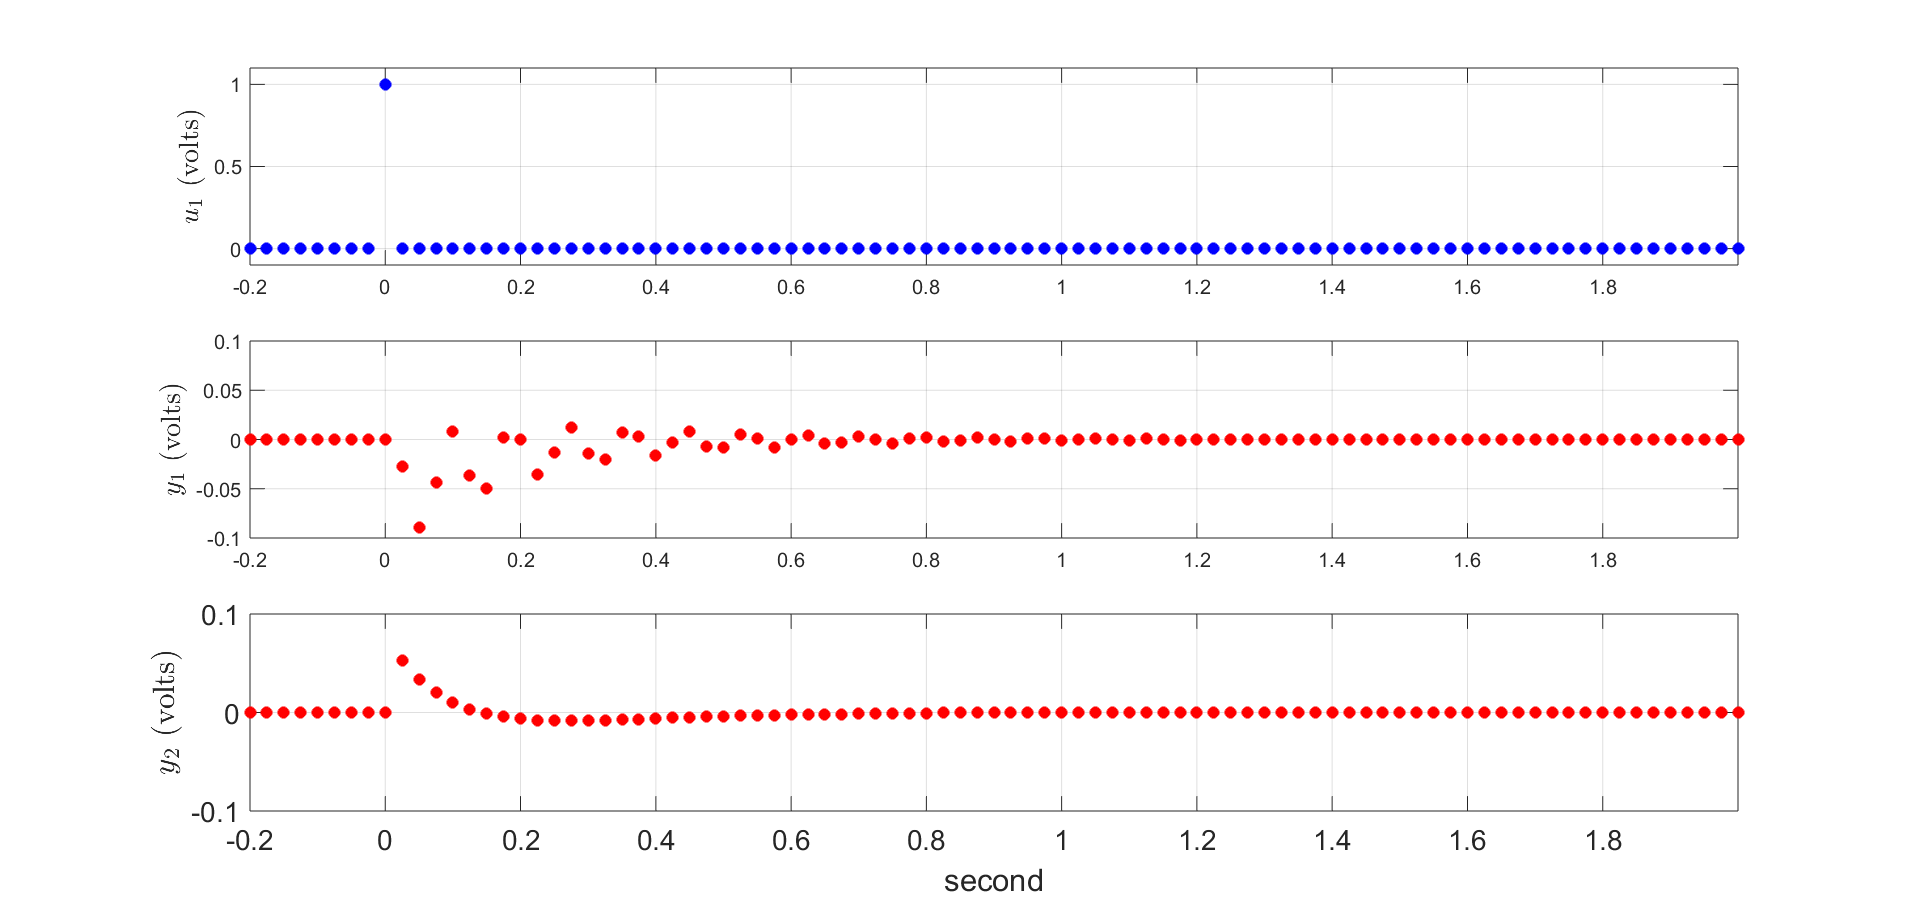
\includegraphics[scale=0.3,trim={4cm 0 0 0},clip]{task01.png}  
		\caption{$u_{1}$ and its corresponding outputs of $y_{1}$ and $y_{2}$  } 
	\end{subfigure}   
	
	\begin{subfigure}{1\textwidth}  
		\centering  
		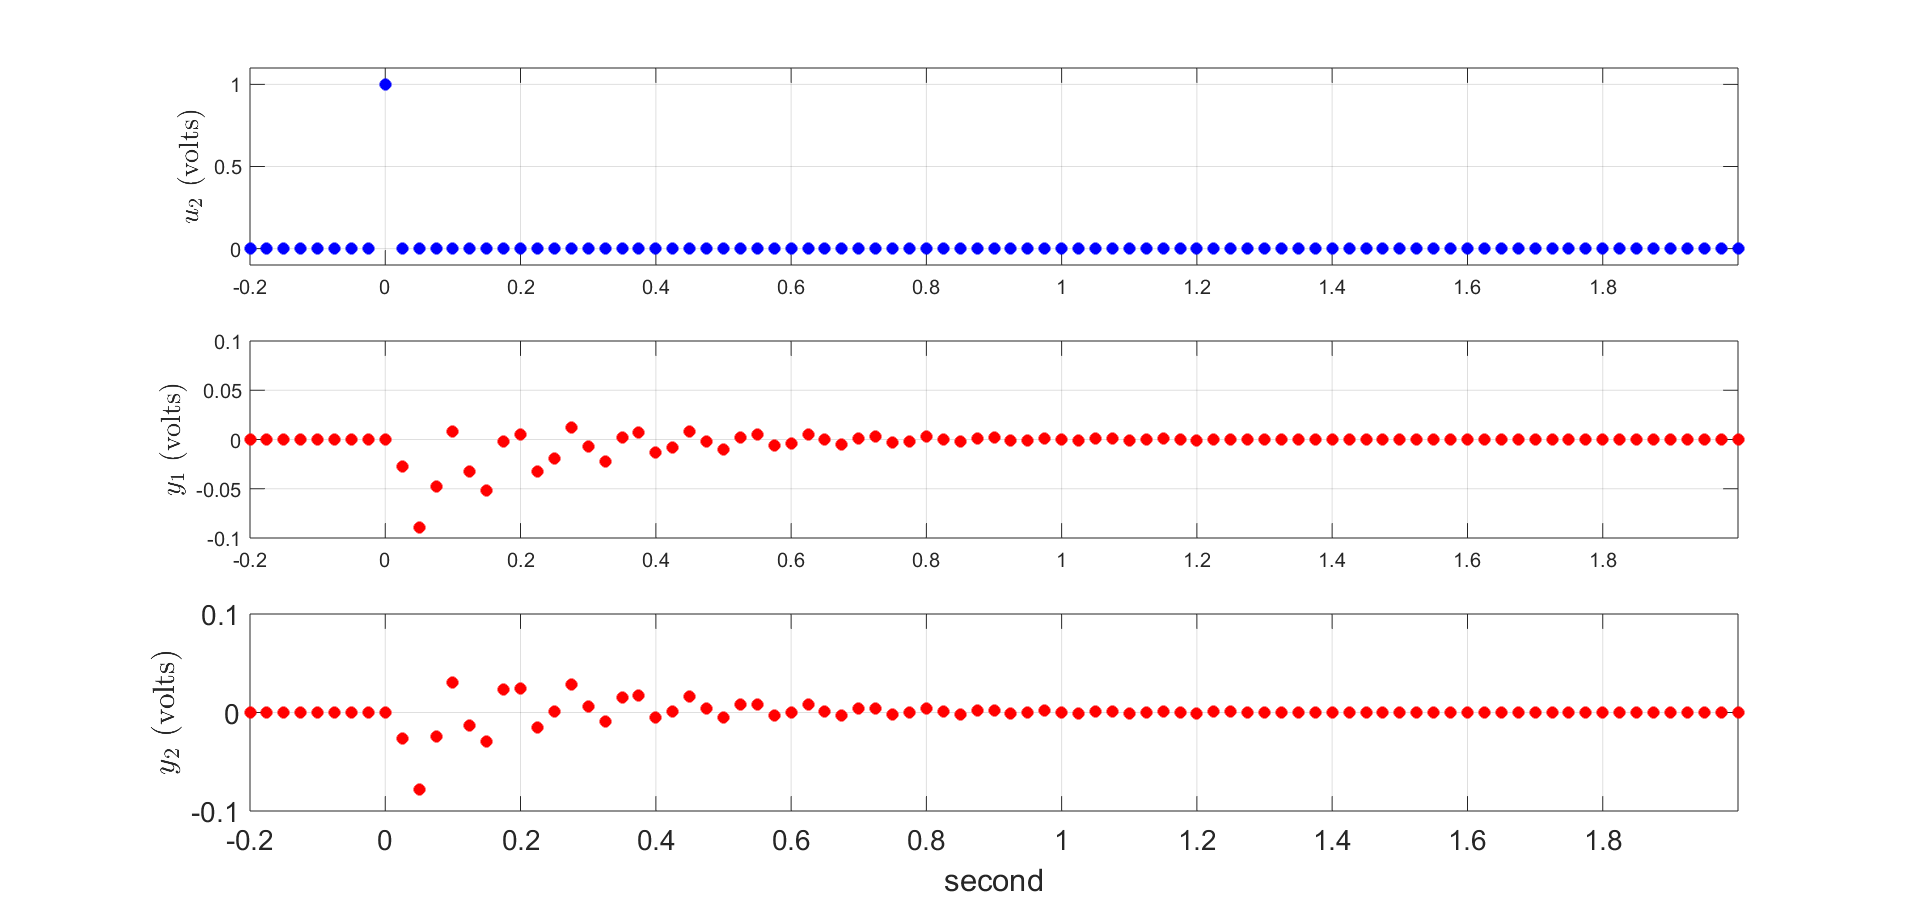
\includegraphics[scale=0.3,trim={4cm 0 0 0},clip]{task02.png}  
		\caption{$u_{2}$ and its corresponding outputs of $y_{1}$ and $y_{2}$  }   
	\end{subfigure}  
	\caption{Actual impulse response of a two-input/two-output system} 
\end{figure} 
\clearpage
\textbf{Task 1: Model Identification}\\
\textbf{1.}\\
In this part we are asked to plot the singular values for $H_{100}$ and compute the models for state dimensions of $n_{s}$ = ${6, 7,10, 20}$. Fig. 2 shows the singular values for $H_{100}$. In this plot we have also included singular values for $H_{20}$, $H_{40}$, and, $H_{80}$ for comparison. Only the first 40 singular values are shown. 


 \begin{figure}[ht!]  
	\centering  
 
		\centering  
		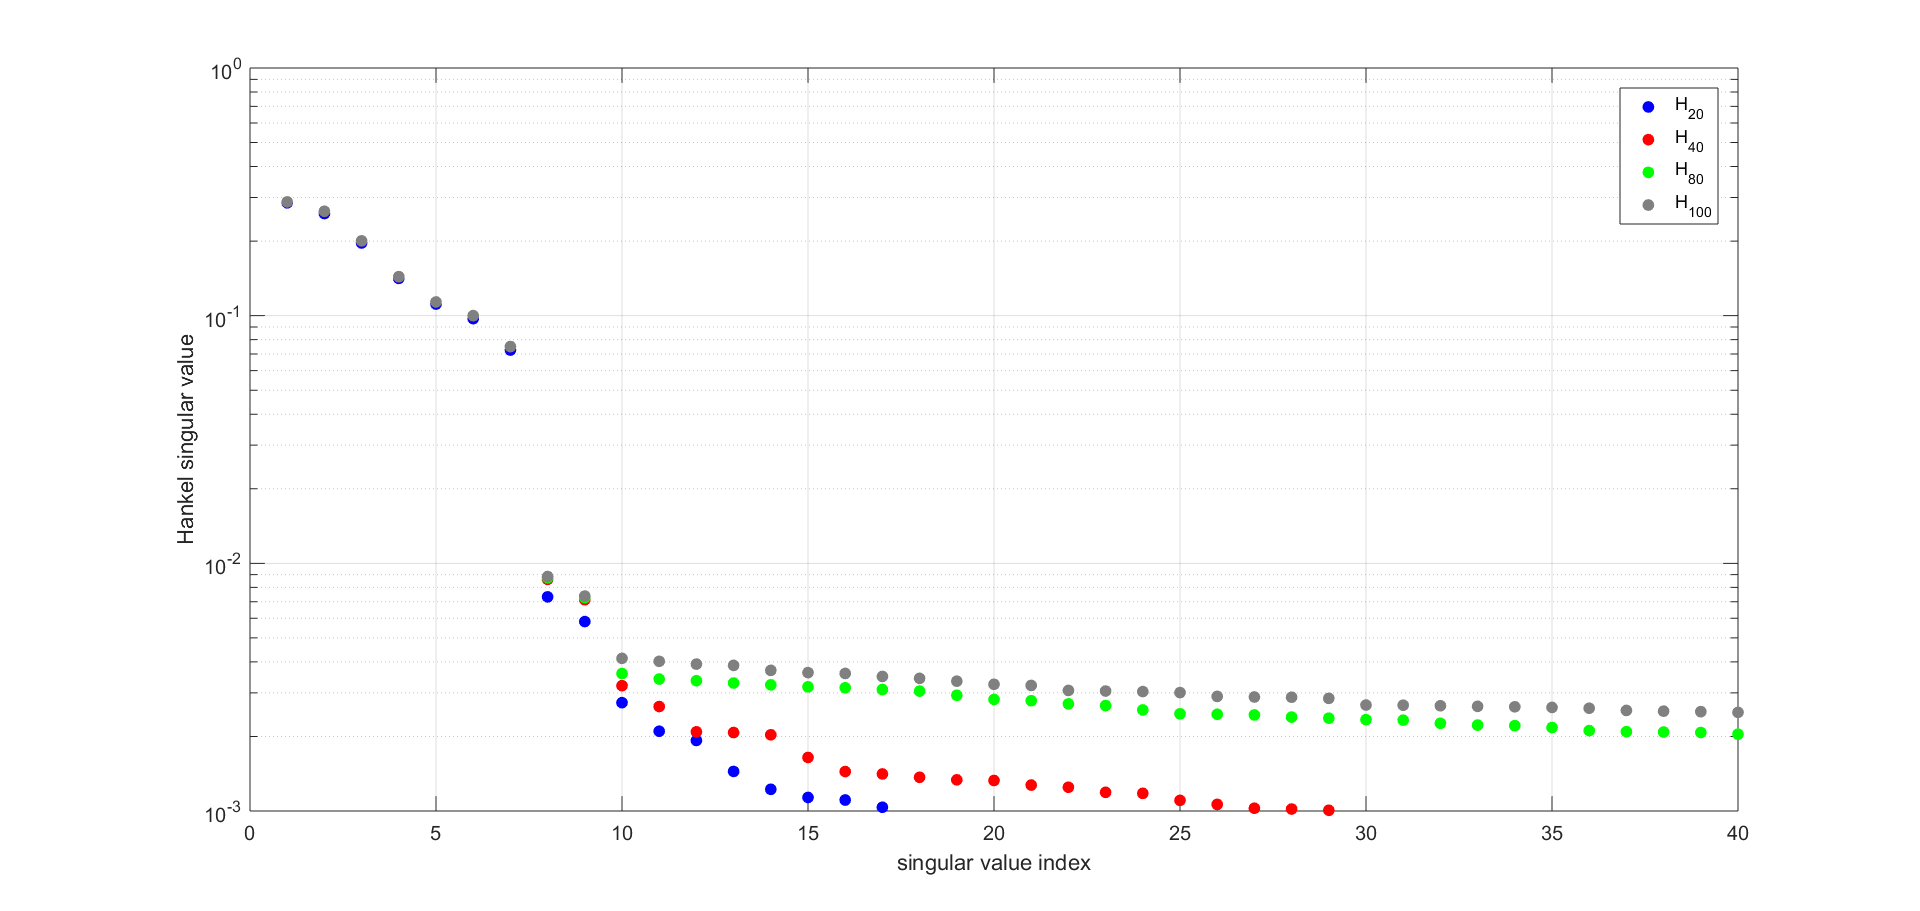
\includegraphics[scale=0.35,trim={4cm 0 0 0},clip]{task11.png}  
		\caption{Hankel singular values} 
  
	%	\caption{Error in the Kalman filter estimates from a single run} 
	\label{task1} 
\end{figure} 


This plot clearly suggests that a good initial choice for the state dimension is $n_{s} = 7$. But we have computed the system's matrices for various $n_{s}$ which will be discussed later. The maximum absolute eigenvalue of the A matrix (computed for $H_{100}$) for each each state dimension are given in Table \ref{eigH100}. Since the numbers for all states are less than 1, it means that all models are asymptotically stable.

\begin{center} \label{eigH100}
	\captionof{table}{Maximum absolute value of the eignevalues for different choice of state dimension}
	\vspace{10pt}
	\begin{tabular}{ |c|c| } 
		\hline
		$n_{s}$ & Max. Abs. of Eigenvalues \\ 
		\hline
		6 & 0.9526 \\ 
		\hline
		7 & 0.9144  \\ 
		\hline
		10 & 0.9141  \\
		\hline 
		20 & 0.9975 \\
		\hline
	\end{tabular}
\end{center}
\vspace{30pt}
\textbf{2.} \\
In this part we are asked to simulate the impulse response (in time domain) for each model with different state dimension. $A$, $B$, $C$ matrices have already been computed for each state dimension of 6, 7, 10,and 20. We should compare these simulated responses with actual impulse response of the system. Fig. 3-6 show the results. 

As it can be seen, the model order of $n_{s}$ = 6 is not able to reproduce the same impulse response as the actual system. The remaining models $n_{s}>>7$ are essentially creating responses that are indistinguishable from the impulse response of the actual system.
\newpage

\begin{figure}[ht!]  
	\centering    
		\centering  
		\includegraphics[scale=0.4,trim={5cm 0 0 0},clip]{task121.png}  
\caption{Simulated vs. actual system response for $n_{s}$ = 6}
	\label{task121} 
\end{figure} 

\begin{figure}[ht!]  
	\centering    
	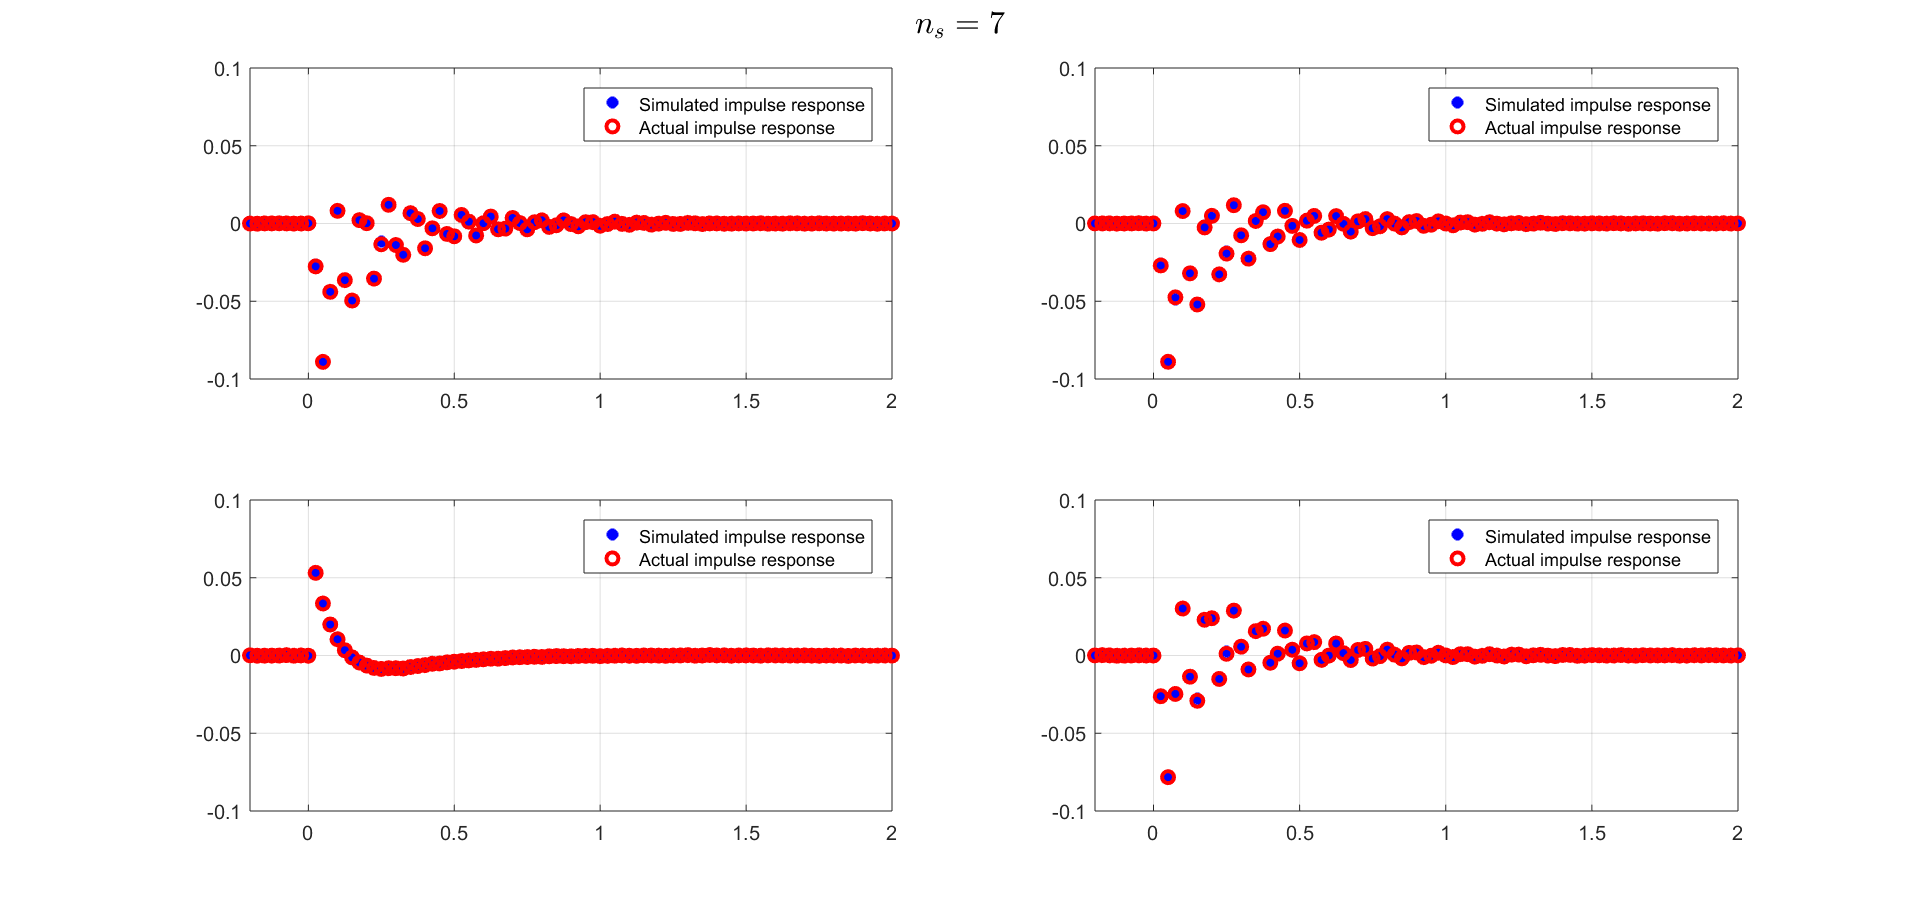
\includegraphics[scale=0.4,trim={5cm 0 0 0},clip]{task122.png}  
\caption{Simulated vs. actual system response for $n_{s}$ = 7}
	\label{task122} 
\end{figure} 


\begin{figure}[ht!]  
	\centering    
	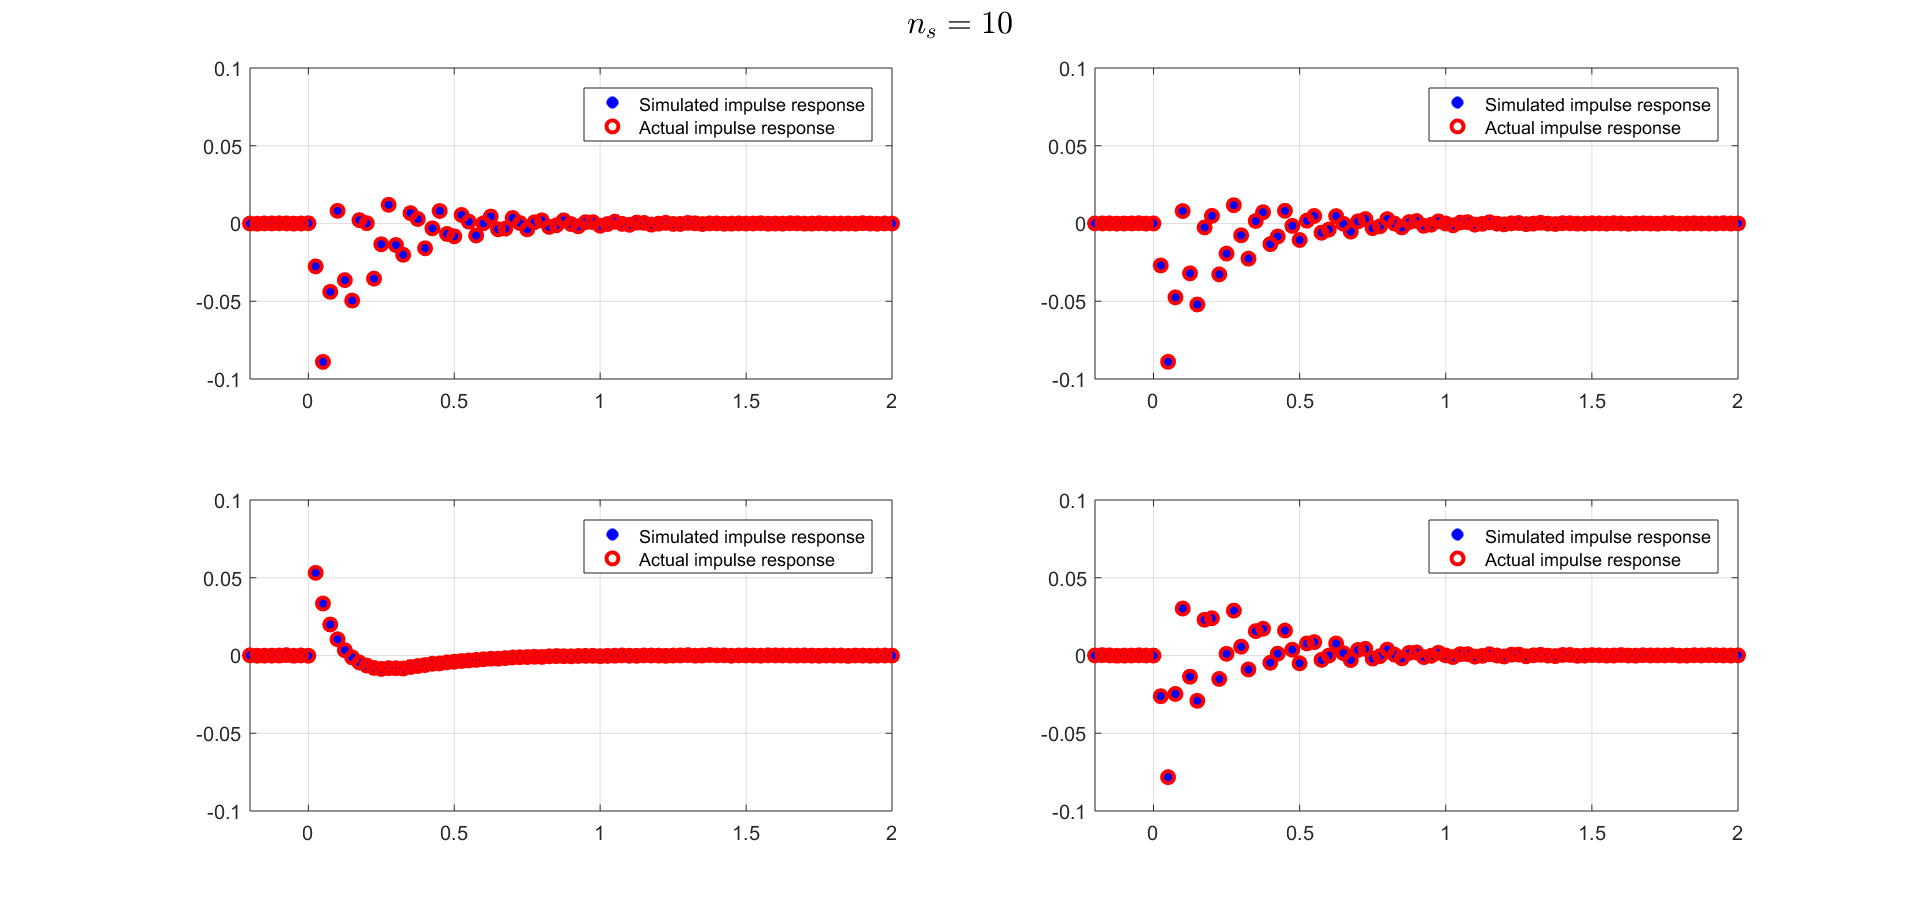
\includegraphics[scale=0.4,trim={5cm 0 0 0},clip]{task123.png}  
\caption{Simulated vs. actual system response for $n_{s}$ = 10}
	\label{task123} 
\end{figure} 


\begin{figure}[ht!]  
	\centering     
	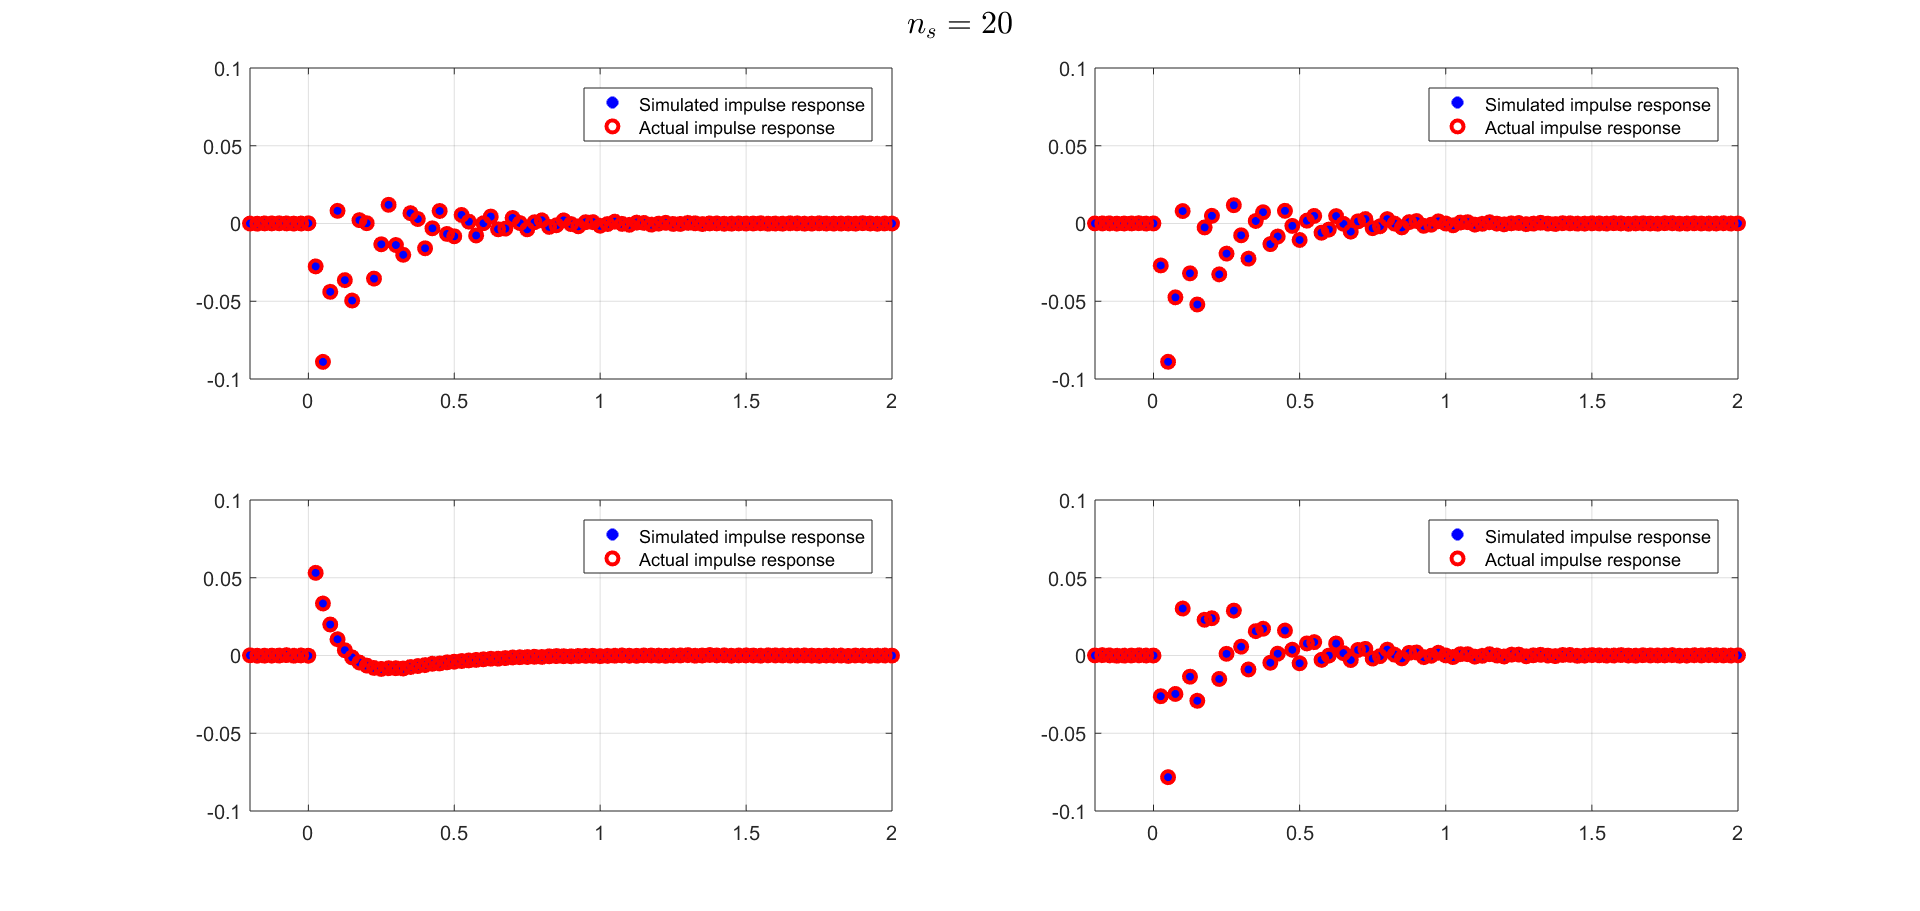
\includegraphics[scale=0.4,trim={5cm 0 0 0},clip]{task124.png}  
	\caption{Simulated vs. actual system response for $n_{s}$ = 20}
	\label{task124} 
\end{figure} 
\clearpage
\textbf{3. \& 4.}

Since parts 3. and 4. are related to the frequency response of the simulated and actual system, we consider them together. 

In this part, comparison between frequency response (as opposed to time-domain response in the previous part) of the model with different state dimensions and the actual system's frequency response is performed. We note that the frequency response of the model is given by:

\begin{gather}
C(e^{jwt_{s}}I-A)^{-1}B+D
\end{gather}

where $t_{s} = 1/40$ is the sampling period in seconds for our data. The frequency $w$ is in the interval of $[0,w_{nyq}]$, where $w_{nyq}$ is the Nyquist frequency (equal to one half of the sampling frequency which is $w_{nyq}$ = 20 hertz or 125.7 rad/s). Note that at each frequency, the frequency response is a $2\times2$ matrix, so we have four complex values at each frequency. For each state dimension with $n_{s} \in \left\{6,7,10,20\right\}$, the magnitude and phase (Bode plot) of each channel are plotted against frequency $w$ in the stated interval. For the magnitude, the log-log plots and for the phase semilog plots are plotted. The corresponding channels, e.g. $(1,1)$ channel for each state dimension are plotted in one figure which would enable us to compare the results across different state dimension.

These frequency responses for each channel are also compared to the responses from actual system. Note that the system's responses is available in the time domain while we need the response in the frequency domain. To do this transformation, the Fast Fourier Transform (FFT) of the output over FFT of the input is used. Similarly, since we have a two-input/two-output system, four channels will be obtained for the empirical data. The corresponding elements to the ones in the model are plotted to compare the responses of the actual and modeled system. Fig. 7-10 demonstrate the results.

As it can be from responses, except the model with dimension $n_{s}=6$ which fails at reproduction of frequency response of the actual data, the other models produce very similar results to the actual system, except that actual system's response are noisy which can be clearly seen in the plots.

The other point to consider in these plots is that basically 3 out of 4 channels have resonant frequencies at around 70 rad/s (i.e., second order system with damping) while the other channel does not. More details on this will be discussed in the next task.

\begin{figure}[ht!]  
	\centering    
	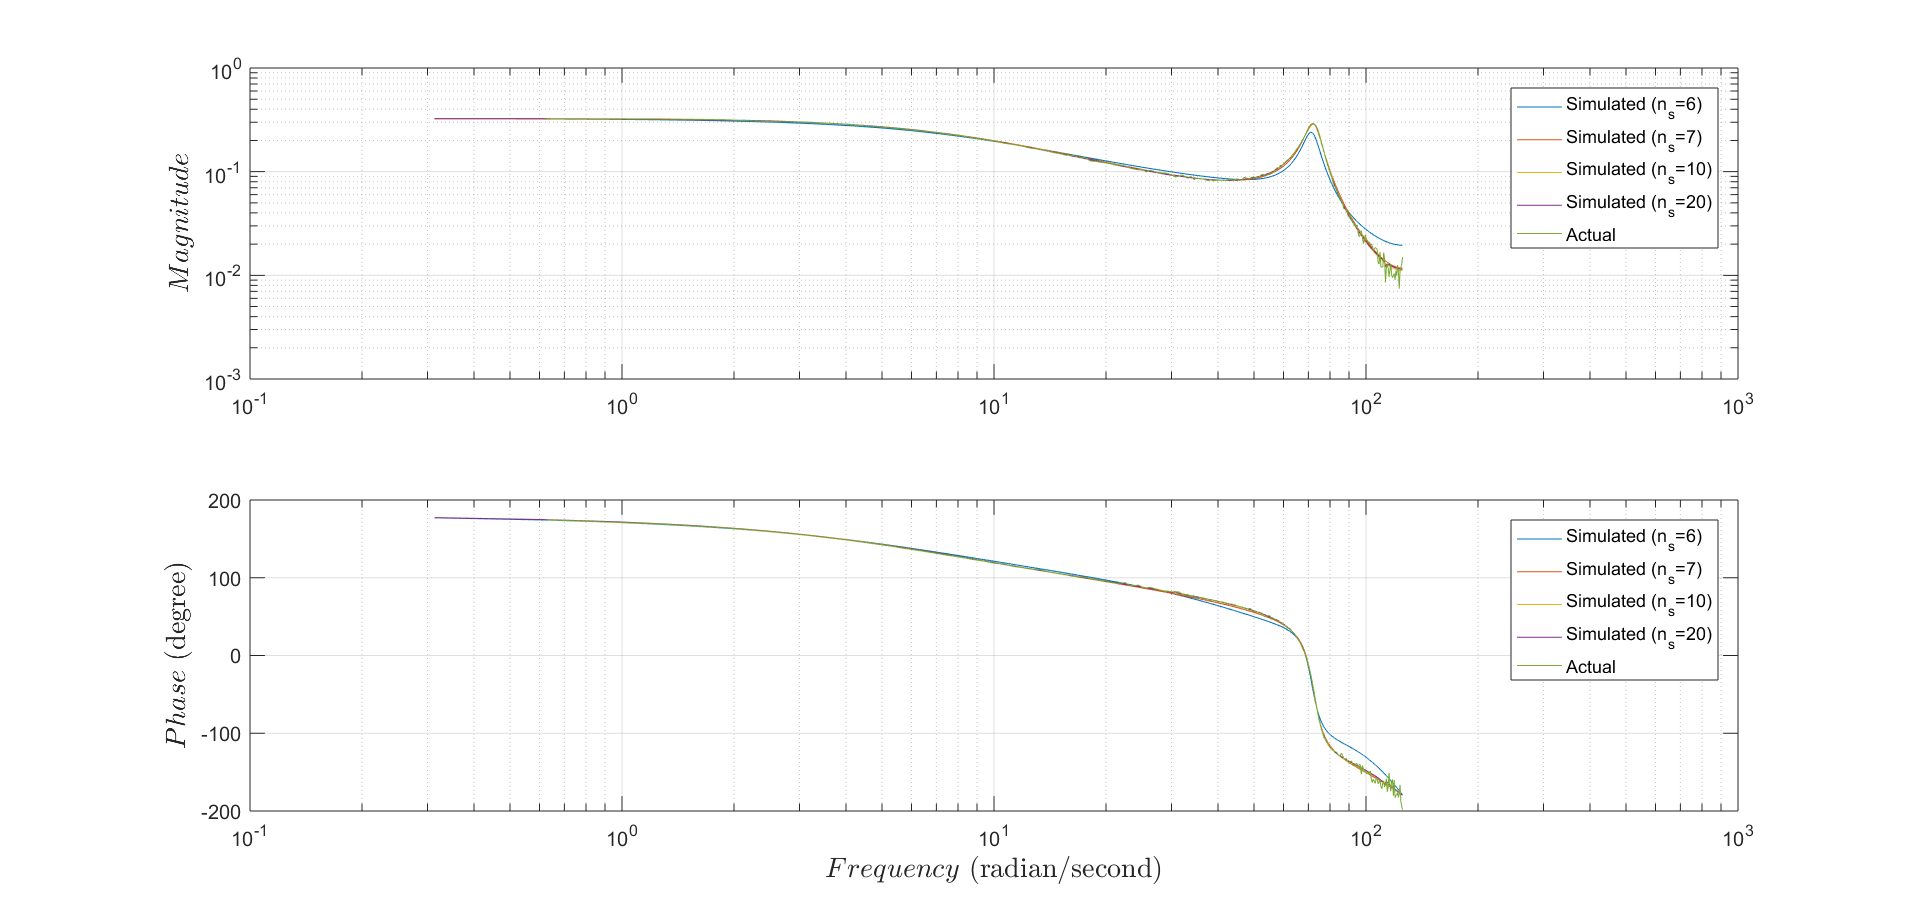
\includegraphics[scale=0.4,trim={5cm 0 0 0},clip]{task131.png}  
	\caption{Bode plot of channel (1,1) for actual system as well as four models with different state dimensions}
	\label{task123} 
\end{figure} 

\begin{figure}[ht!]  
	\centering    
	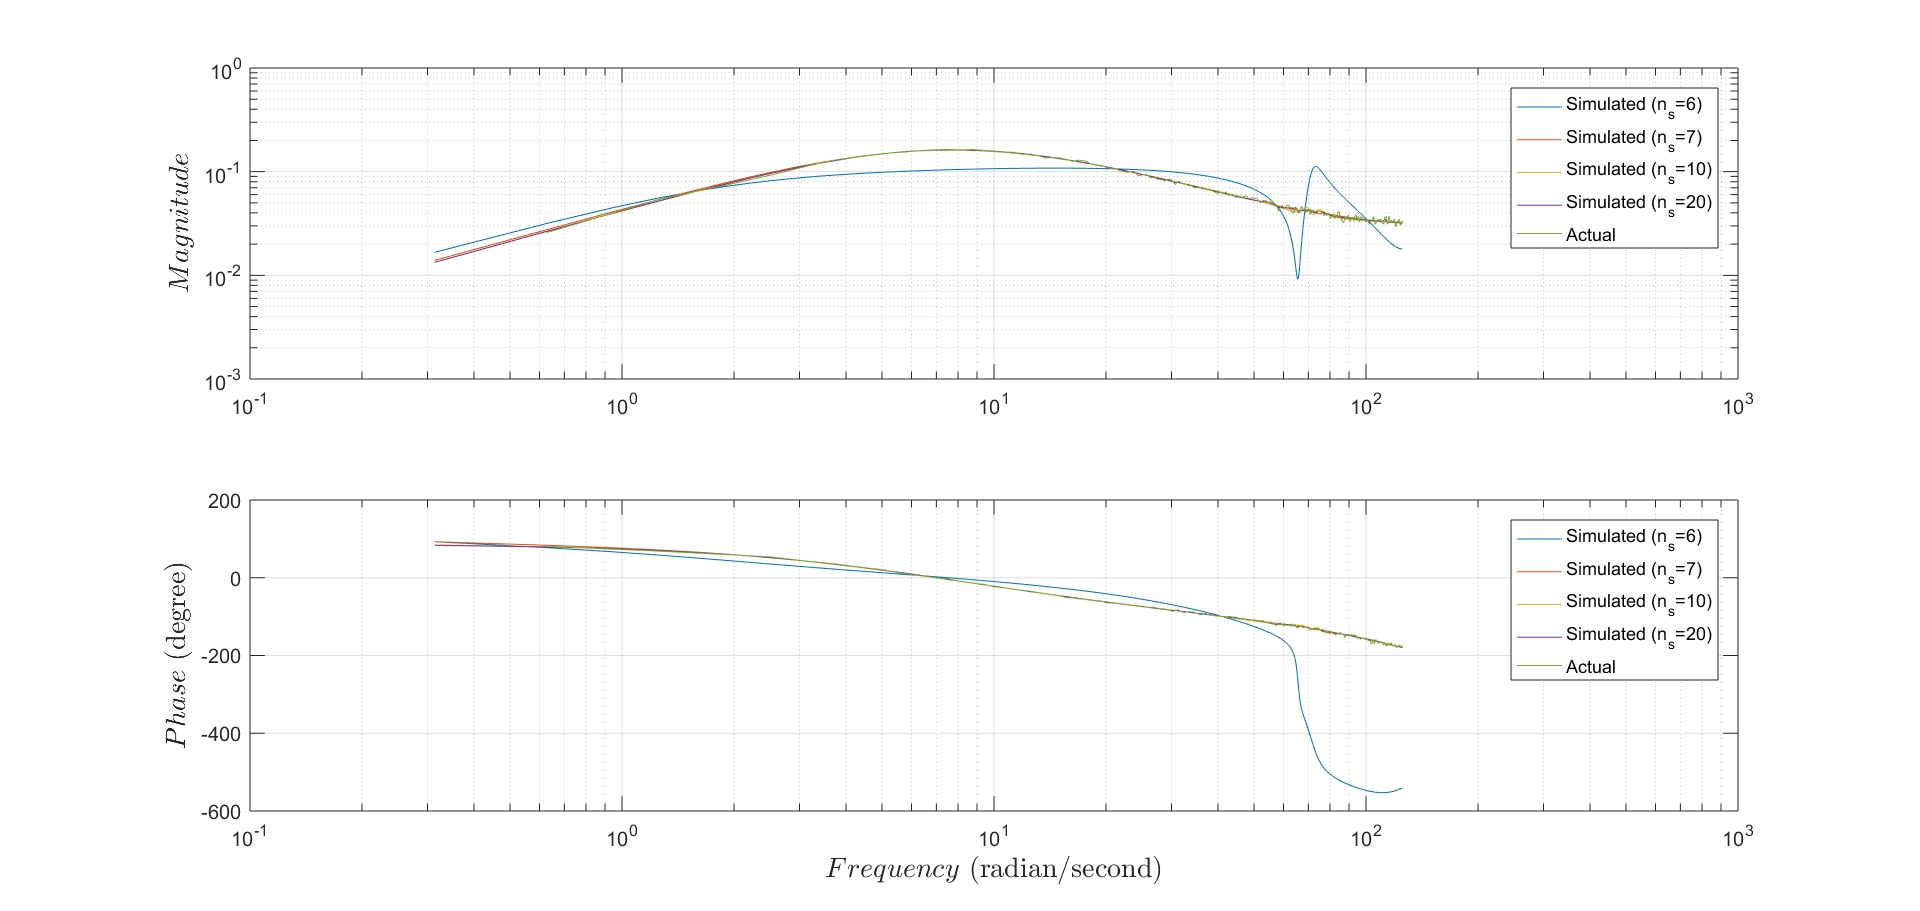
\includegraphics[scale=0.4,trim={5cm 0 0 0},clip]{task132.png}  
	\caption{Bode plot of channel (2,1) for actual system as well as four models with different state dimensions}
	\label{task123} 
\end{figure} 

\begin{figure}[ht!]  
	\centering    
	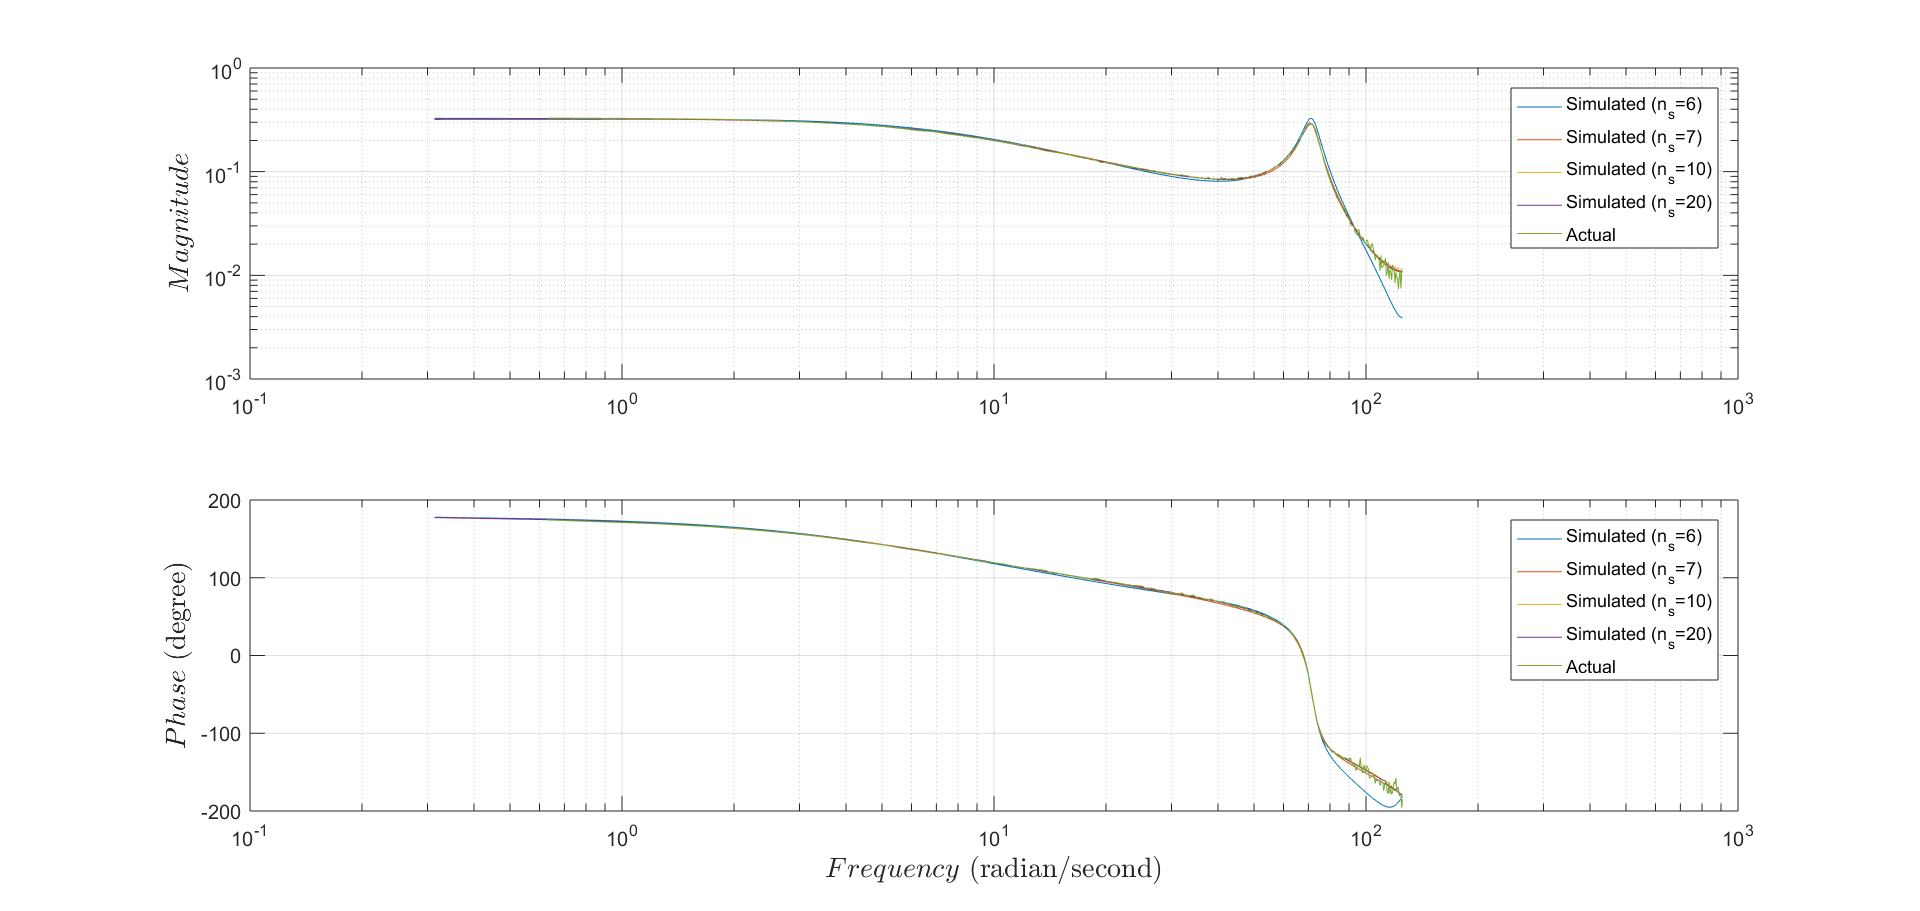
\includegraphics[scale=0.4,trim={5cm 0 0 0},clip]{task133.png}  
	\caption{Bode plot of channel (1,2) for actual system as well as four models with different state dimensions}
	\label{task123} 
\end{figure} 

\begin{figure}[ht!]  
	\centering    
	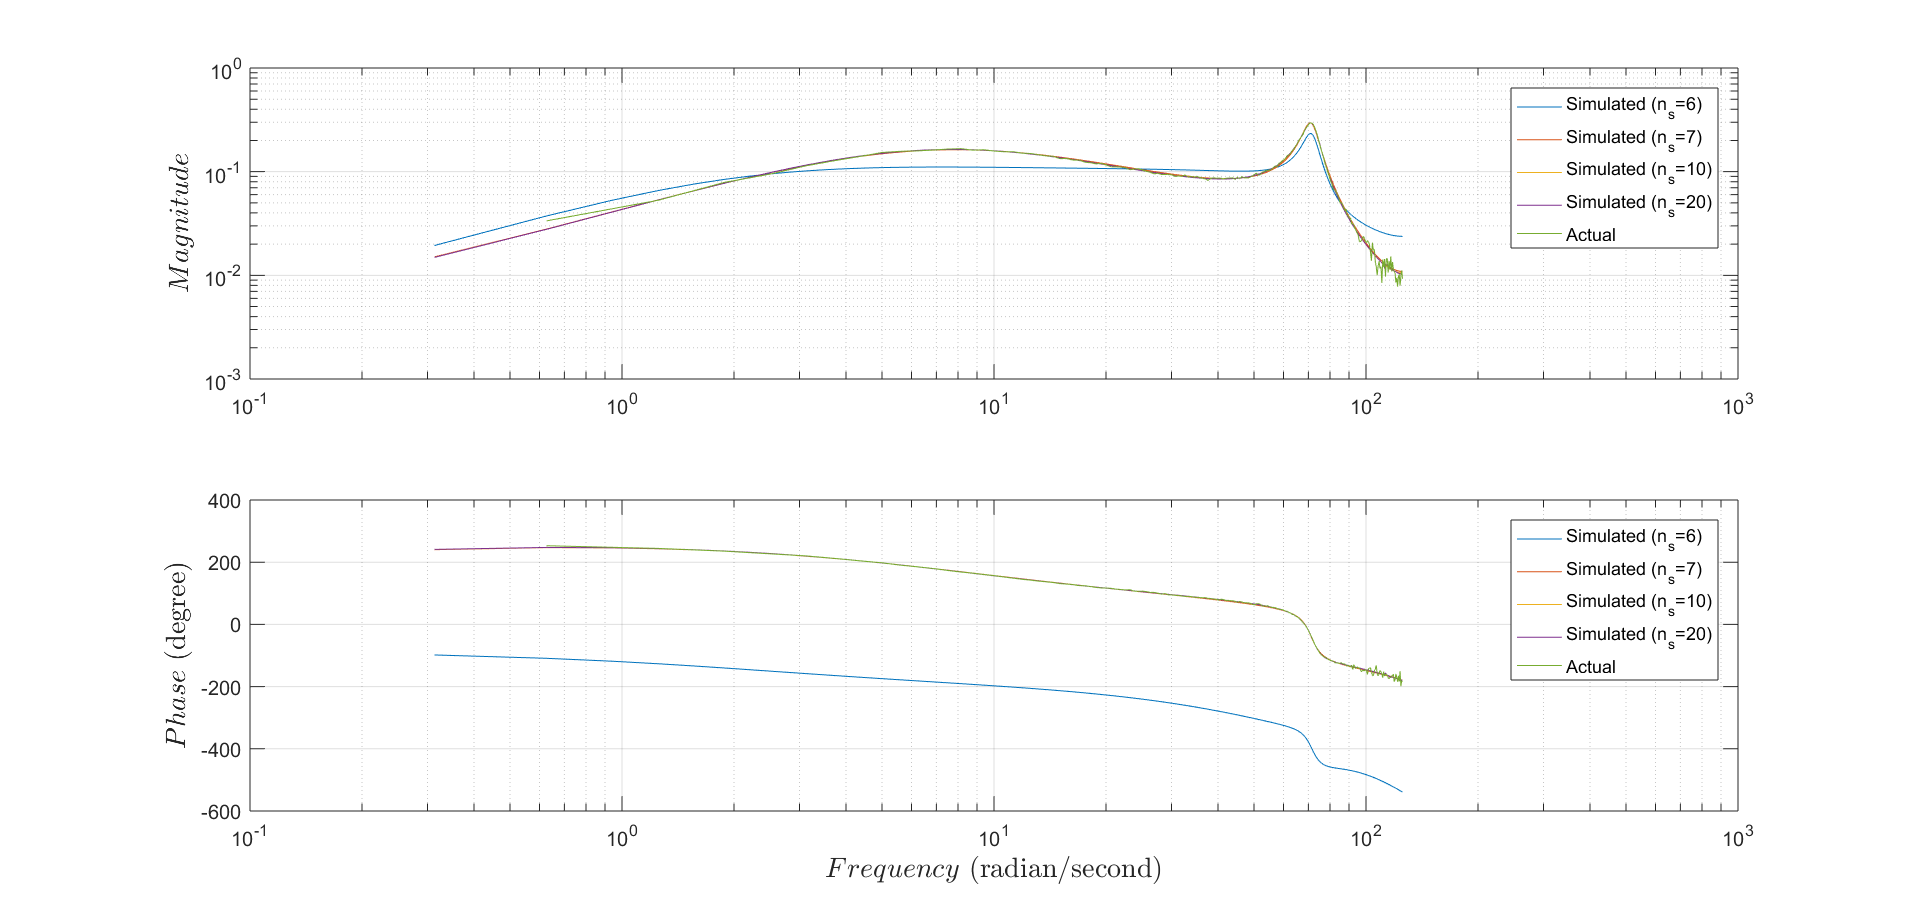
\includegraphics[scale=0.4,trim={5cm 0 0 0},clip]{task134.png}  
	\caption{Bode plot of channel (2,2) for actual system as well as four models with different state dimensions}
	\label{task123} 
\end{figure} 

\clearpage
\textbf{Task 2: Transmission zeros of the MIMO model and zeros of each channel}

In this section we want to compute the transmission zeros of the model we obtained from previous section. The models with state dimension of $n_{s}=7,8$ which provide a very accurate model of the actual system (in terms of both time and frequency responses) are considered in this task. For calculating the zeros of the system, a generalized eigenvalue problem are used according to the following relation:

\begin{gather*}
 \begin{bmatrix}
A & B \\
-C & -D \\
\end{bmatrix} \tag{2}
\begin{bmatrix}
\textbf{c} \\
\textbf{w} \\
\end{bmatrix} = z
\begin{bmatrix}
I & 0\\
0 & 0 \\
\end{bmatrix} \begin{bmatrix}
\textbf{c} \\
\textbf{w} \\
\end{bmatrix}
\end{gather*}

It is quite straightforward to show that if the system has a transmission zero $z \in \textbf{C}$, then the exists initial condition $\textbf{c} \in \textbf{C}^{7}$, and input $\textbf{w} \in \textbf{C}^{2}$, $\textbf{u}_{k}$ = $\textbf{w}z^{k}$ such that the output remains zero for all samples.

The other point that we know about the transmission zeros are that they do not have to appear in the numerator of any transfer function of each channel. In this regard, it is harder, compared to system's poles, to find system's zeros and/or intuitively guess them.

\vspace{30pt}
\textbf{1.} \\
For this task we are asked to compute the transmission zeros of the model with $n_{s}$ = 7. Eq. 2 was used in Matlab to calculate the zeros of the system. In this case four of the zeros are "inf" which can be ignored. The remaining five are list in the Table 2. The 'sort' command in Matlab was used to sort the eigenvalues from largest to smallest magnitude.

\begin{center} \label{eigH100}
	\captionof{table}{Transmission zeros of the model with 7 state dimension.}
	\vspace{10pt}
	\begin{tabular}{ |c|c| } 
		\hline
		index & Transmission zeros ($n_{s}=7$) \\ 
		\hline
		$z_{1}$ & -2.6310 \\
		\hline
		$z_{2}$ & 0.9988   \\ 
		\hline
		$z_{3}$ & -0.6078 + 0.6740j \\
		\hline 
	    $z_{4}$ & -0.6078 - 0.6740j \\
		\hline
		$z_{5}$ & -0.3241 \\
		 \hline
	\end{tabular}
\end{center}

\vspace{20pt}
$z_{1}$ is called an unstable zeros as $|z_{1}|>1$ and the input it generates is unbounded. As it can be seen, for all other zeros we have $|z_{p}|<1$, $p=2,3,4,5$ and they are asymptotically stable poles because the input they generate decays to zero.\\

\vspace{30pt}
\textbf{2.}\\
In this part, we are asked to plot both of the eigenvalues and zeros on the complex plane. As we know, the stability of a discrete dynamic system is obtained when the magnitude of all the eigenvalues is less than 1, in other words, when all the eigenvalues remain inside the unit circle in the complex plane. Since all of the eigenvalues remain inside the unit circle (see Fig. \ref{task22}), the system is asymptotically stable.

\begin{figure}[ht!]  
	\centering    
	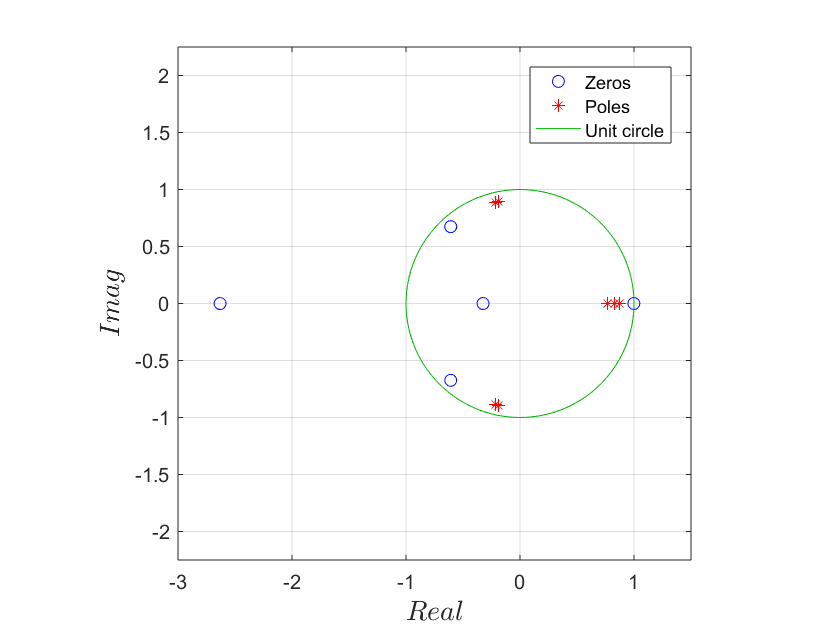
\includegraphics[scale=0.6,trim={1cm 0 0 0},clip]{task22.png}  
	\caption{eigenvalues/zeros of 7-state model}
	\label{task22} 
\end{figure} 
\vspace{30pt}
\textbf{3.}\\
In this task we are asked to convent the discrete-time eigenvalue computed from previous parts to its 'equivalent' continuous-time eigenvalue. The relationship between eigenvalues of continuous- and discrete-time can be expressed as:

\begin{gather}
\lambda_{d} = e^{\lambda_{c}t_{s}}
\tag{3}
\end{gather} 

Note that from this relationship, $\lambda_{d}$ is not uniquely defined since: 

\begin{gather*}
\lambda_{d} = e^{\lambda_{c}t_{s}}\\
\lambda_{c}' = \lambda_{c} + 2\pi\frac{k}{t_{s}}j, \text{ }k = \pm1,\pm2,... \\ 
\Rightarrow e^{\lambda_{c}'t_{s}} = e^{(\lambda_{c}+2\pi\frac{k}{t_{s}}j)t_{s}} = e^{\lambda_{c}t_{s}}e^{2\pi kj} = e^{\lambda_{c}t_{s}} = \lambda_{d}
\tag{4}
\end{gather*} 


These relationships show that the imaginary part of $\lambda_{c}$ is not uniquely defined, so we just pick the one with smallest value. The set of computed $\lambda_{c}$'s are displayed in Table 3.

\begin{center} \label{eigH100}
	\captionof{table}{Maximum absolute value of the eignevalues for different choice of state dimension}
	\vspace{10pt}
	\begin{tabular}{ |c| } 
		\hline
		$\lambda_{c}$ \\ 
		\hline
		  -3.6842 +71.1394j \\
		  \hline
		-3.6842 -71.1394j \\
		\hline
		-3.5800 +72.2737j \\
		\hline
		-3.5800 -72.2737j \\
		\hline
		-10.4604 \\
		\hline
		-7.6568 \\
		\hline
		-5.6364 \\ 
		\hline
	\end{tabular}
\end{center}

\vspace{20pt}
As it can be seen from the computed values of $\lambda_{c}$'s, we can see that there are two damped oscillators in our model at frequencies of 71.13 and 72.27 Hz. Interestingly, these frequencies do show up in our frequency response plots as well. As it can be seen in Fig. 7, Fig. 9, and Fig. 10, the magnitude of frequency response in these plots experience a peak at frequencies around 70 Hz which is a feature for second order system with damping. Note that, however, only one peak is seen in these plots while the results from computing $\lambda_{c}$ suggest that two peaks are expected for each channel. This explicitly suggest that for these channel we expect that a pair of zeros should be close to one pair of oscillatory eigenvalues (the ones with non-zeros imaginary part) and due to pole/zero cancellation only one resonant frequency be appeared. Note that there is no resonant frequency (peak in magnitude) available for the other channel displayed Fig. 8. These issues will be examined in the next part.

\vspace{30pt}
\textbf{4.}\\
In this section we are asked to plot the calculated eigenvalues and transmission zeros for each of the four channels separately and essentially treating each channel as a separate single-input/single-out system. Fig. \ref{task241}-\ref{task244} depict the eigenvalues/zeros on the complex plane as well as the Hankel singular values (from $H_{100}$) for each channel.

The first point consider in this part is that basically the eigenvalues for each channel are equal and the difference between them are transmission zeros. As explained previously, from computed $\lambda_{c}$ we would expect to see two resonant frequencies in the response but we only see one in three plots (Fig. 7, Fig. 9, Fig. 10) and non in the other plot (Fig. 8). 
As it can be seen in Fig. 12, for this channel, there are 6 transmission zeros and seven eigenvalues. As demonstrated before and also can be seen here, 2 pairs of eigenvalues have imaginary part (it is hard to these pairs on the plot since they are very close to each other) and three have only real part. Four our of six transmission zeros on are real axis, two of which are very close to the eigenvalues and hence, we have pole/zero cancellation for them. More importantly, the pair of transmission zeros that have imaginary part are very close to the two pairs of eigenvalues, canceling the effect of one pair (pole/zero cancellation). Hence, effectively this channel has only one pair of poles/eigenvalues with imaginary part (oscillatory) which is why we only see one peak in the frequency response and not two. Very similar arguments can be made for other two channels which have one resonant frequency and a pole/zero cancellation for one pair of eigenvalues with imaginary part (Fig. 14, and Fig. 15). For the other channel (see Fig. 8) in which there is no resonant frequency in the response, Fig. 13 shows that, in addition for one pole/zero cancellation on the real axis, both pairs of oscillatory eigenvalues (non-zero imaginary part) are canceled by two pairs of transmission zeros which are very close to those eigenvalues and hence no effects of oscillations will be in the frequency response (no peak in Fig. 8). 

As it can be seen, each plot (Fig. 12-15) which corresponds to each channel in isolation also includes the corresponding Hankel singular values. For instance, in Fig. 12 it can be noted that there is a significant jump between the third and fourth singular value suggesting that this channel can be well approximated with the third order system. This results also matches with the corresponding plots of eigenvalues/zeros on the complex plane. Although there are 7 eigenvalues for this channel, the effects of four of them (two on the real axis and one pair with non-zero imaginary part) is canceled due to pole/zero cancellation, and hence effectively this channel can be well approximated with a third order system. A similar analysis can be done for other channels as well. The channels plotted in Fig. 13-15 can be a well approximated with a second, third, and fourth order system respectively.

\begin{figure}[bh!]  
	\centering    
	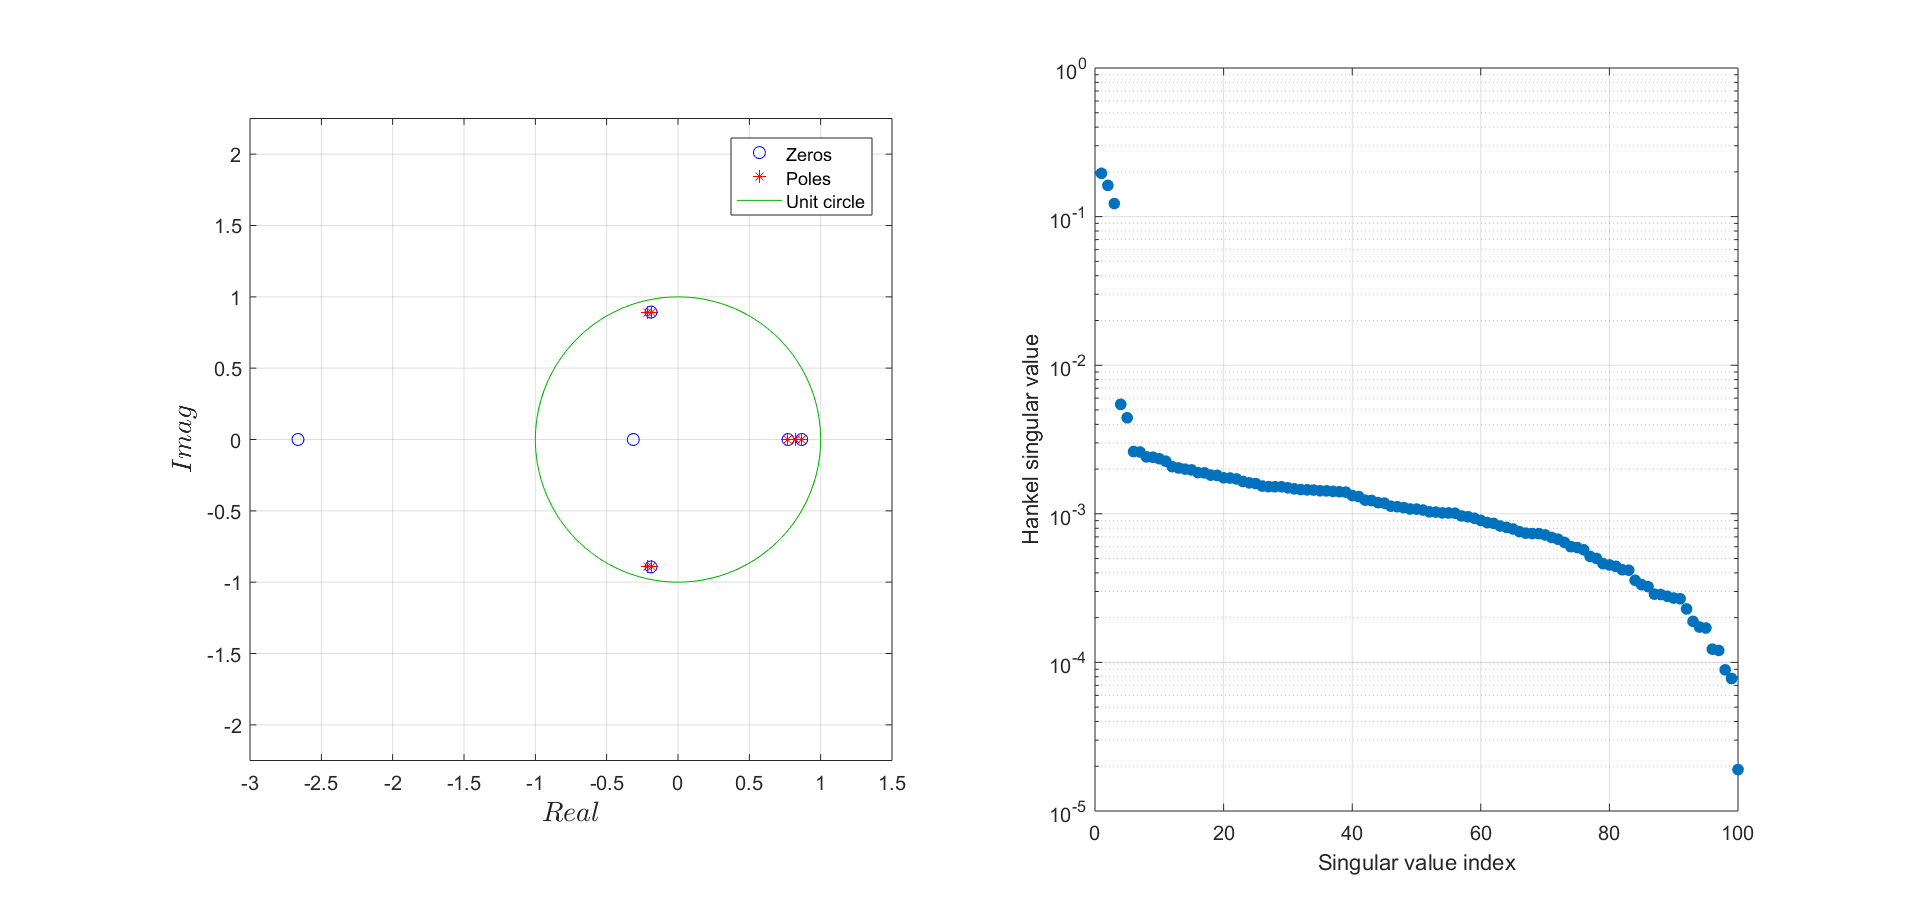
\includegraphics[scale=0.38,trim={4.5cm 0 0 0},clip]{task241.png}  
	\caption{eigenvalues/zeros of 7-state model for channel $(1,1)$}
	\label{task241} 
\end{figure} 

\begin{figure}[ht!]  
	\centering    
	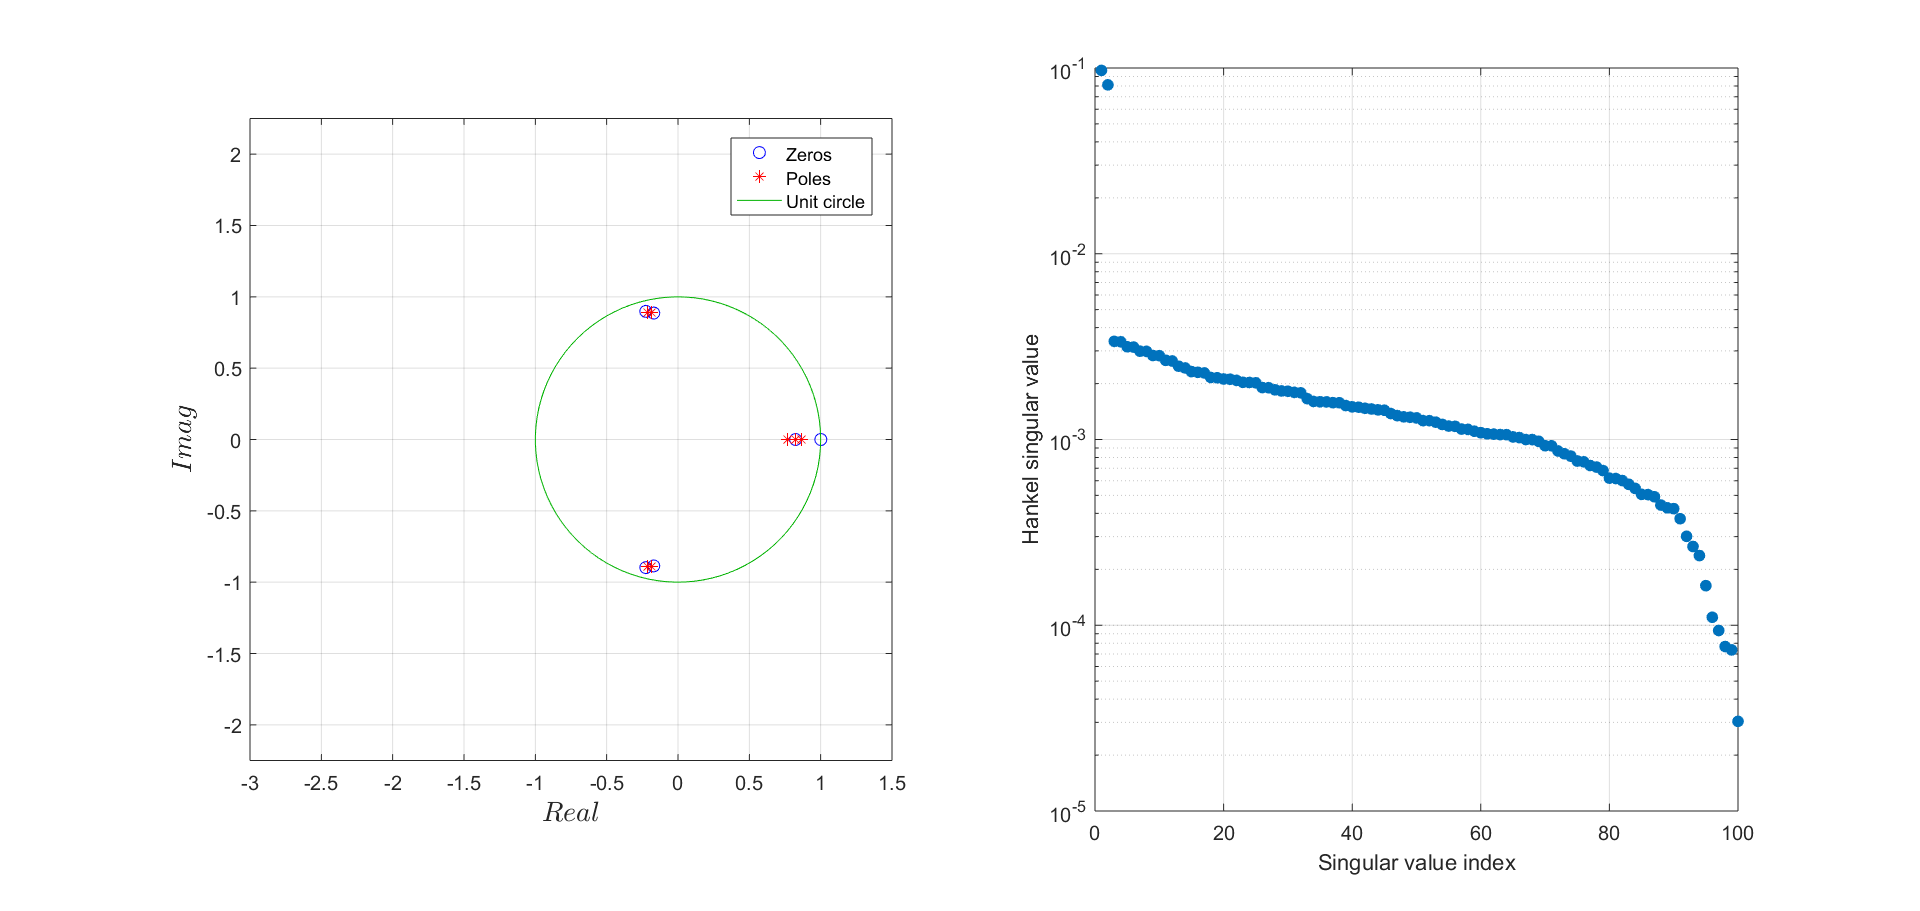
\includegraphics[scale=0.38,trim={4.5cm 0 0 0},clip]{task242.png}  
	\caption{eigenvalues/zeros of 7-state model for channel $(2,1)$}
	\label{task242} 
\end{figure} 

\begin{figure}[ht!]  
	\centering    
	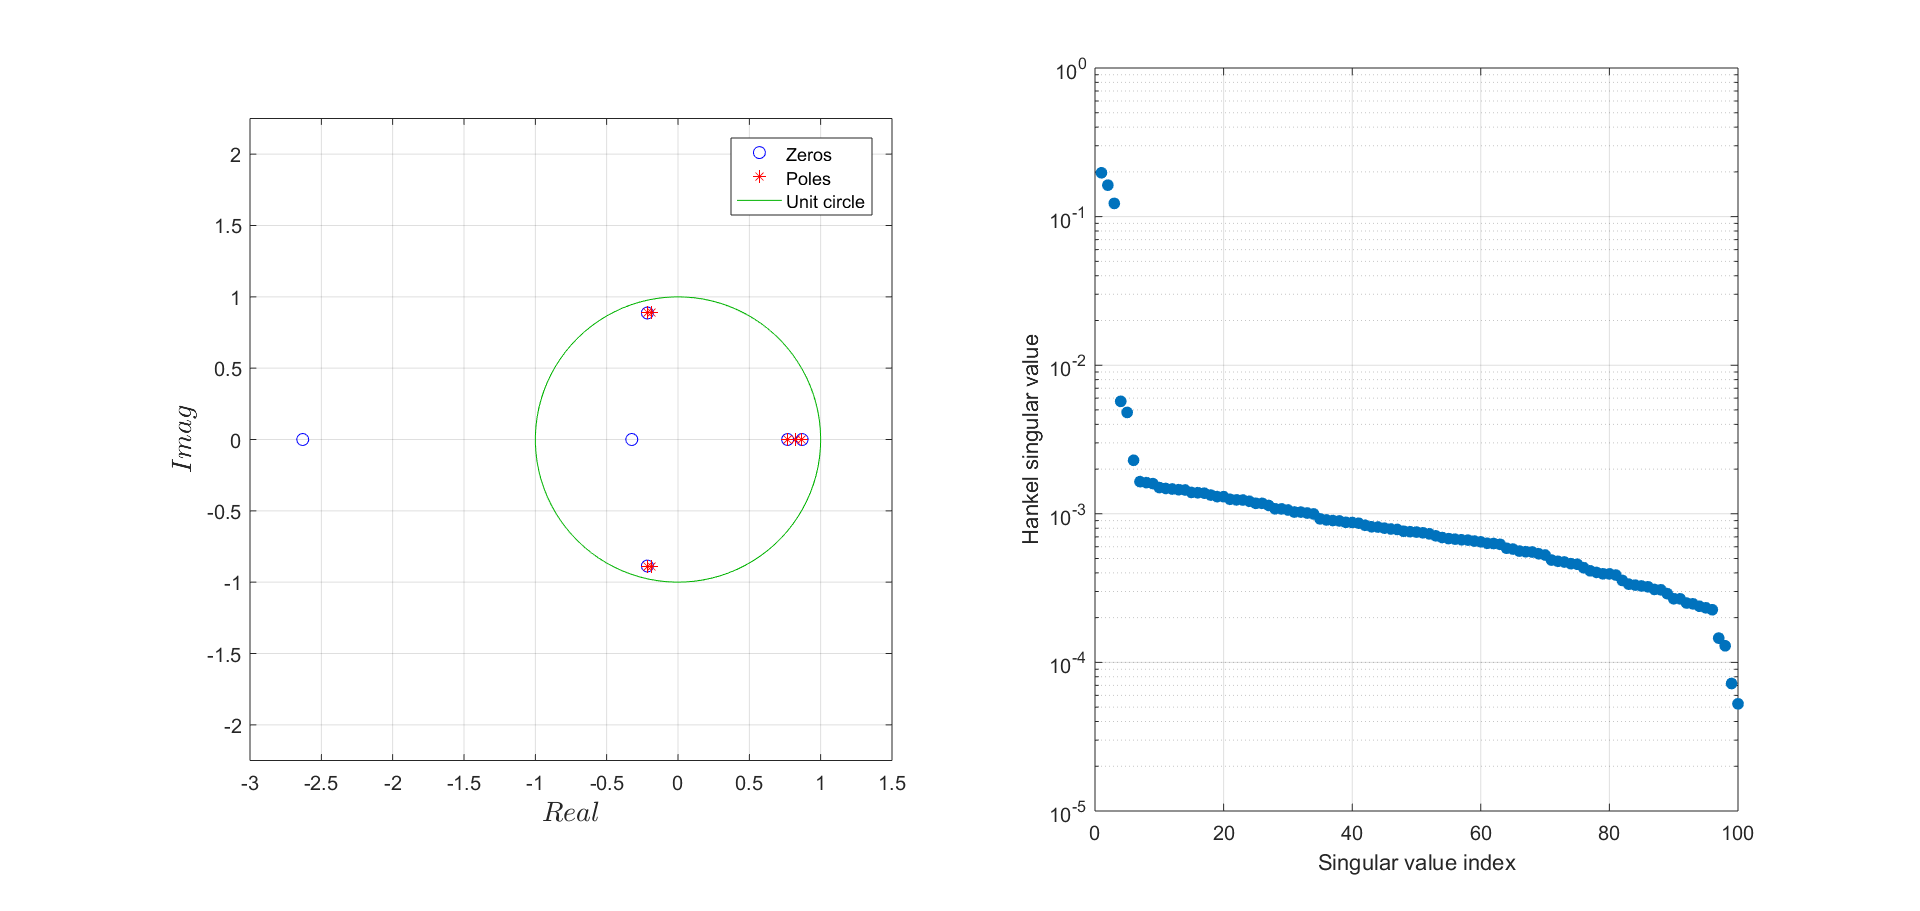
\includegraphics[scale=0.38,trim={4.5cm 0 0 0},clip]{task243.png}  
	\caption{eigenvalues/zeros of 7-state model for channel $(1,2)$}
	\label{task243} 
\end{figure} 

\begin{figure}[t!]  
	\centering    
	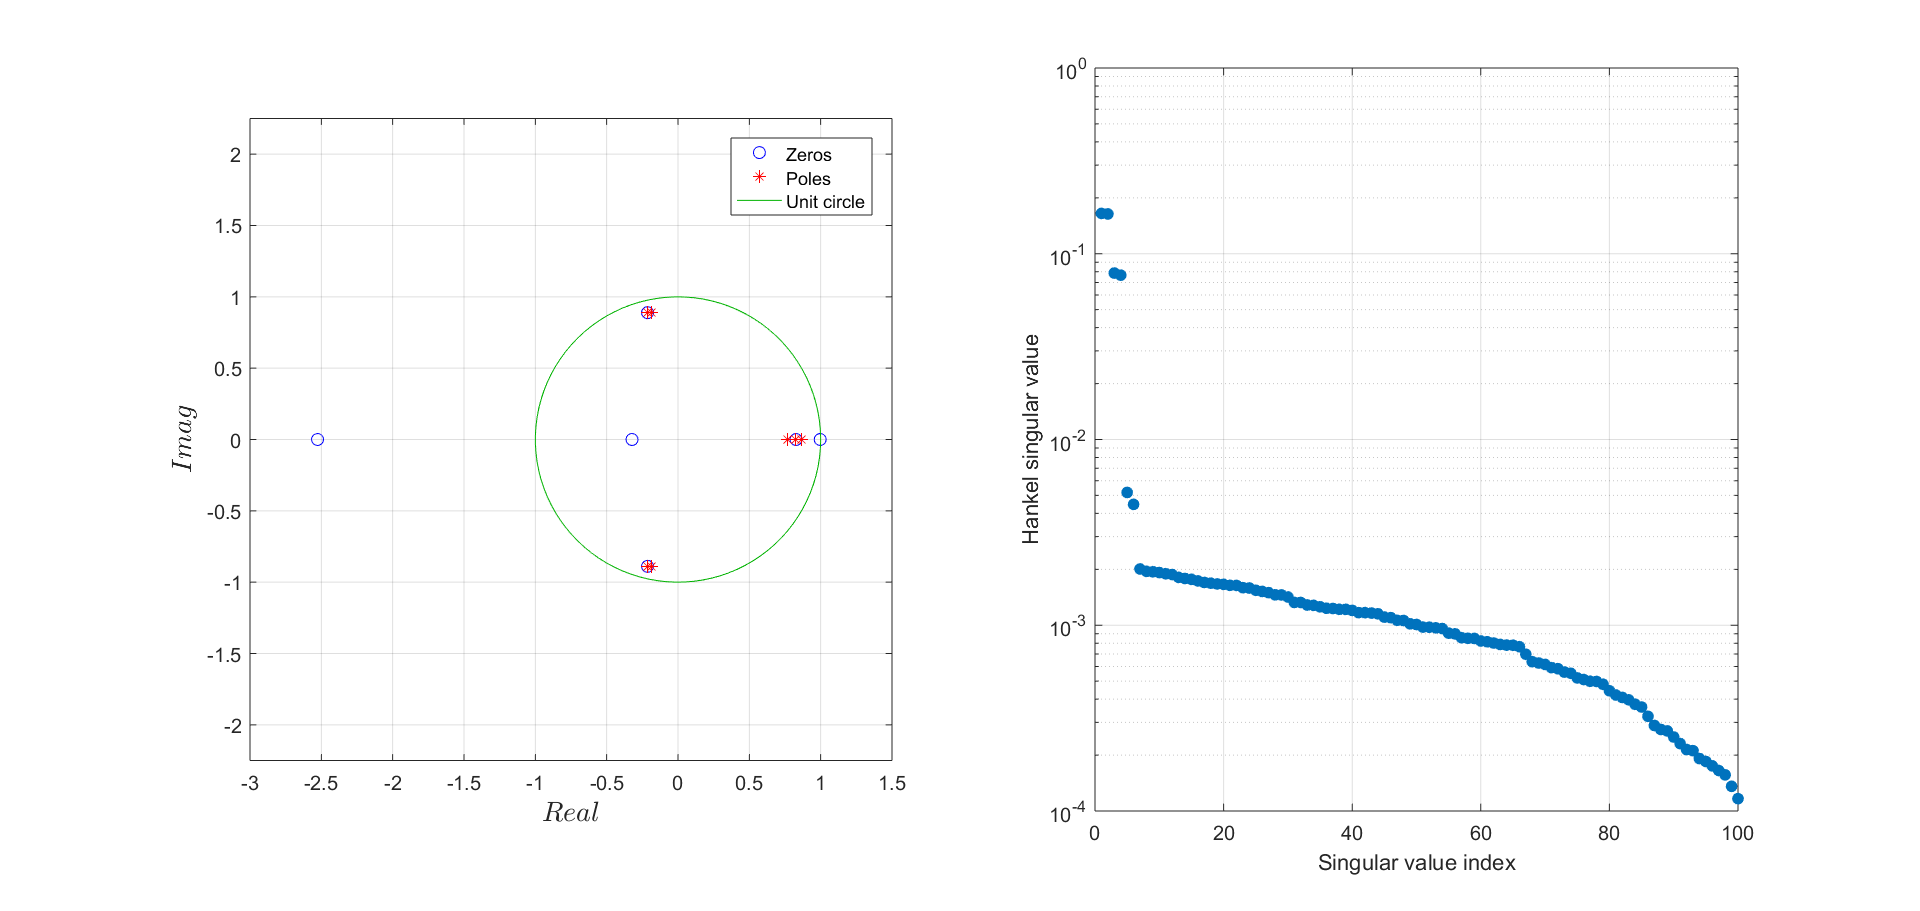
\includegraphics[scale=0.38,trim={4.5cm 0 0 0},clip]{task244.png}  
	\caption{eigenvalues/zeros of 7-state model for channel $(2,2)$}
	\label{task244} 
\end{figure} 
\clearpage
\textbf{5.}\\
In this part, we are asked to plot the eigenvalues and transmission zeros for the model with state dimension $n_{s}=8$. Since the impulse response of the model and the model with $n_{s}=7$, it is essentially over-parametrized meaning that the existence of additional dimension does not provide a 'better' model. Hence, such information should somehow be explained by comparing the eigenvalues/zeros of both models on the complex plane.
 


\begin{figure}[bh!]  
	\centering    
	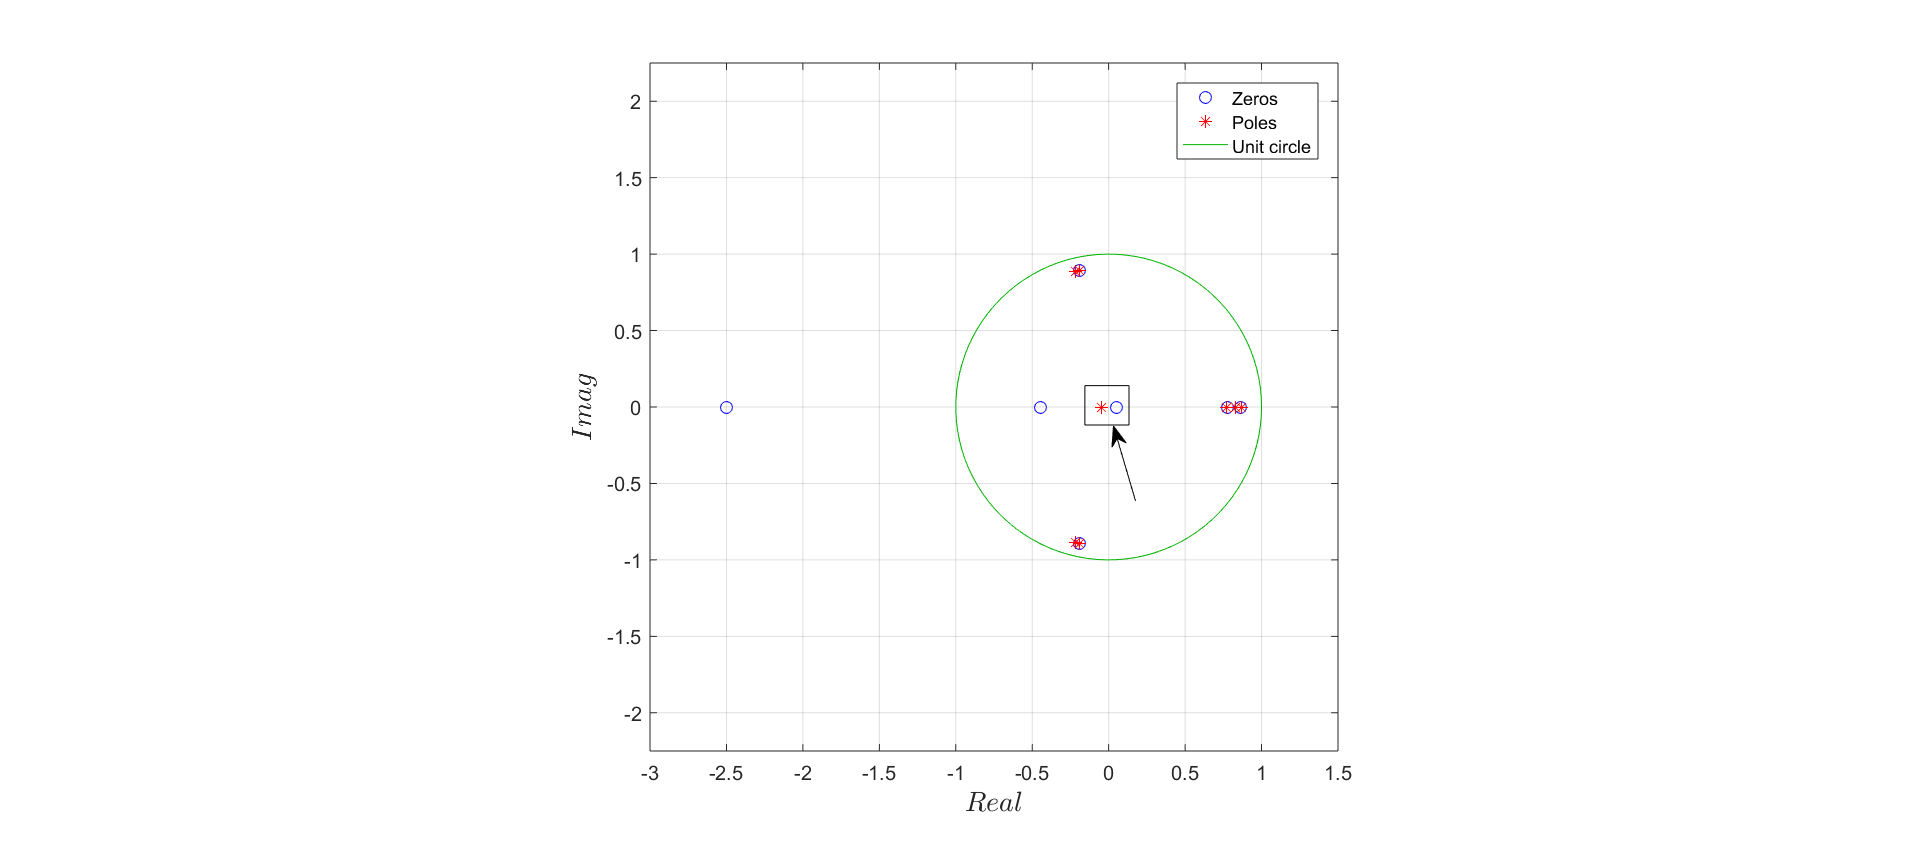
\includegraphics[scale=0.38,trim={4.5cm 0 0 0},clip]{task251.png}  
	\caption{eigenvalues/zeros of 8-state model for channel $(1,1)$}
	\label{task251} 
\end{figure} 

\begin{figure}[ht!]  
	\centering    
	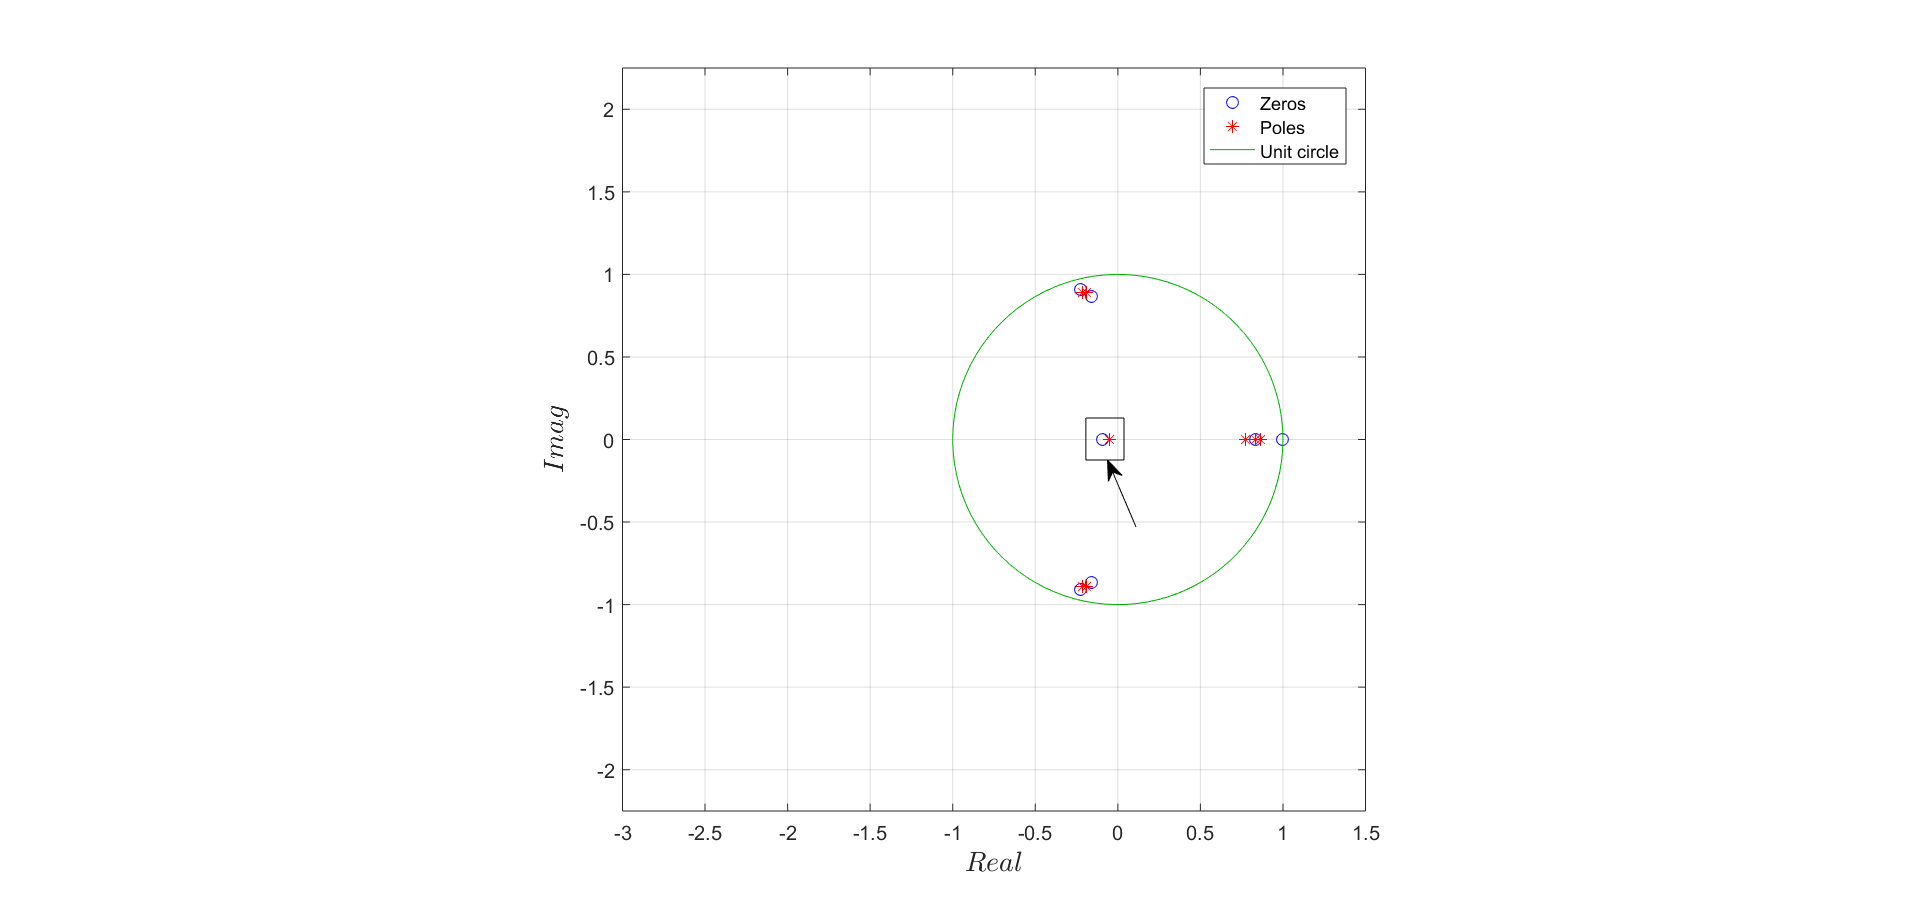
\includegraphics[scale=0.38,trim={4.5cm 0 0 0},clip]{task253.png}  
	\caption{eigenvalues/zeros of 8-state model for channel $(2,1)$}
	\label{task252} 
\end{figure} 

\begin{figure}[ht!]  
	\centering    
	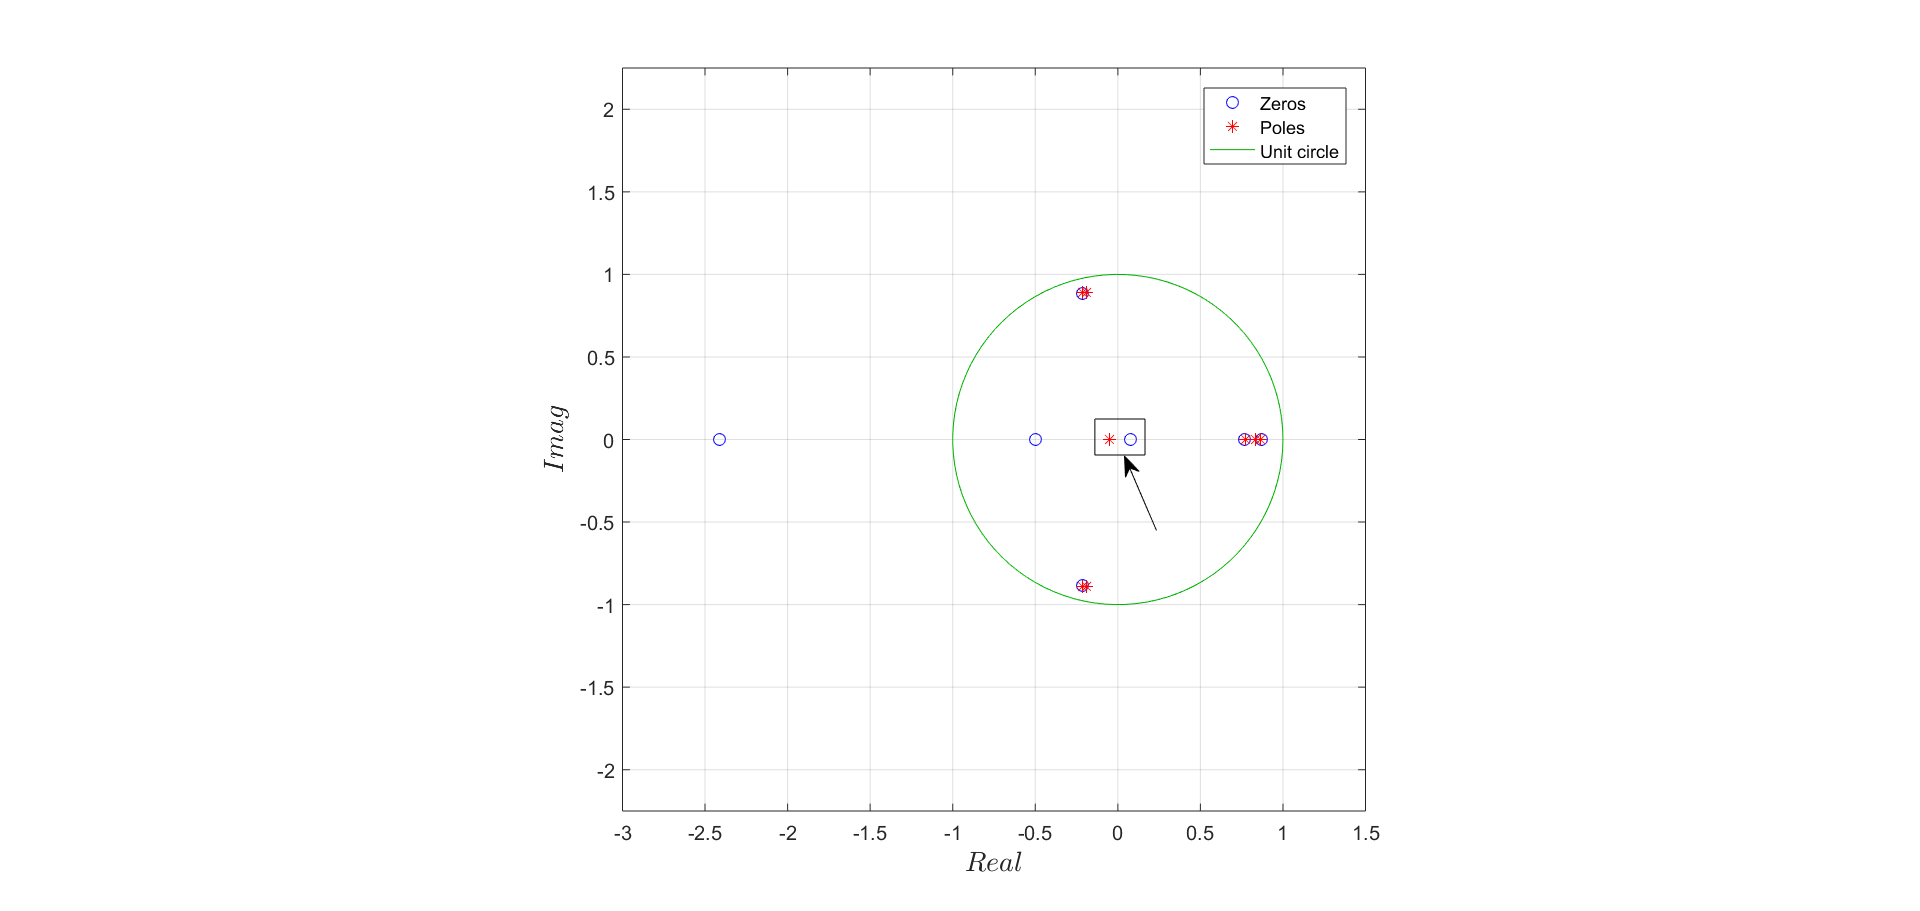
\includegraphics[scale=0.38,trim={4.5cm 0 0 0},clip]{task252.png}  
	\caption{eigenvalues/zeros of 8-state model for channel $(1,2)$}
	\label{task253} 
\end{figure} 

\begin{figure}[t!]  
	\centering    
	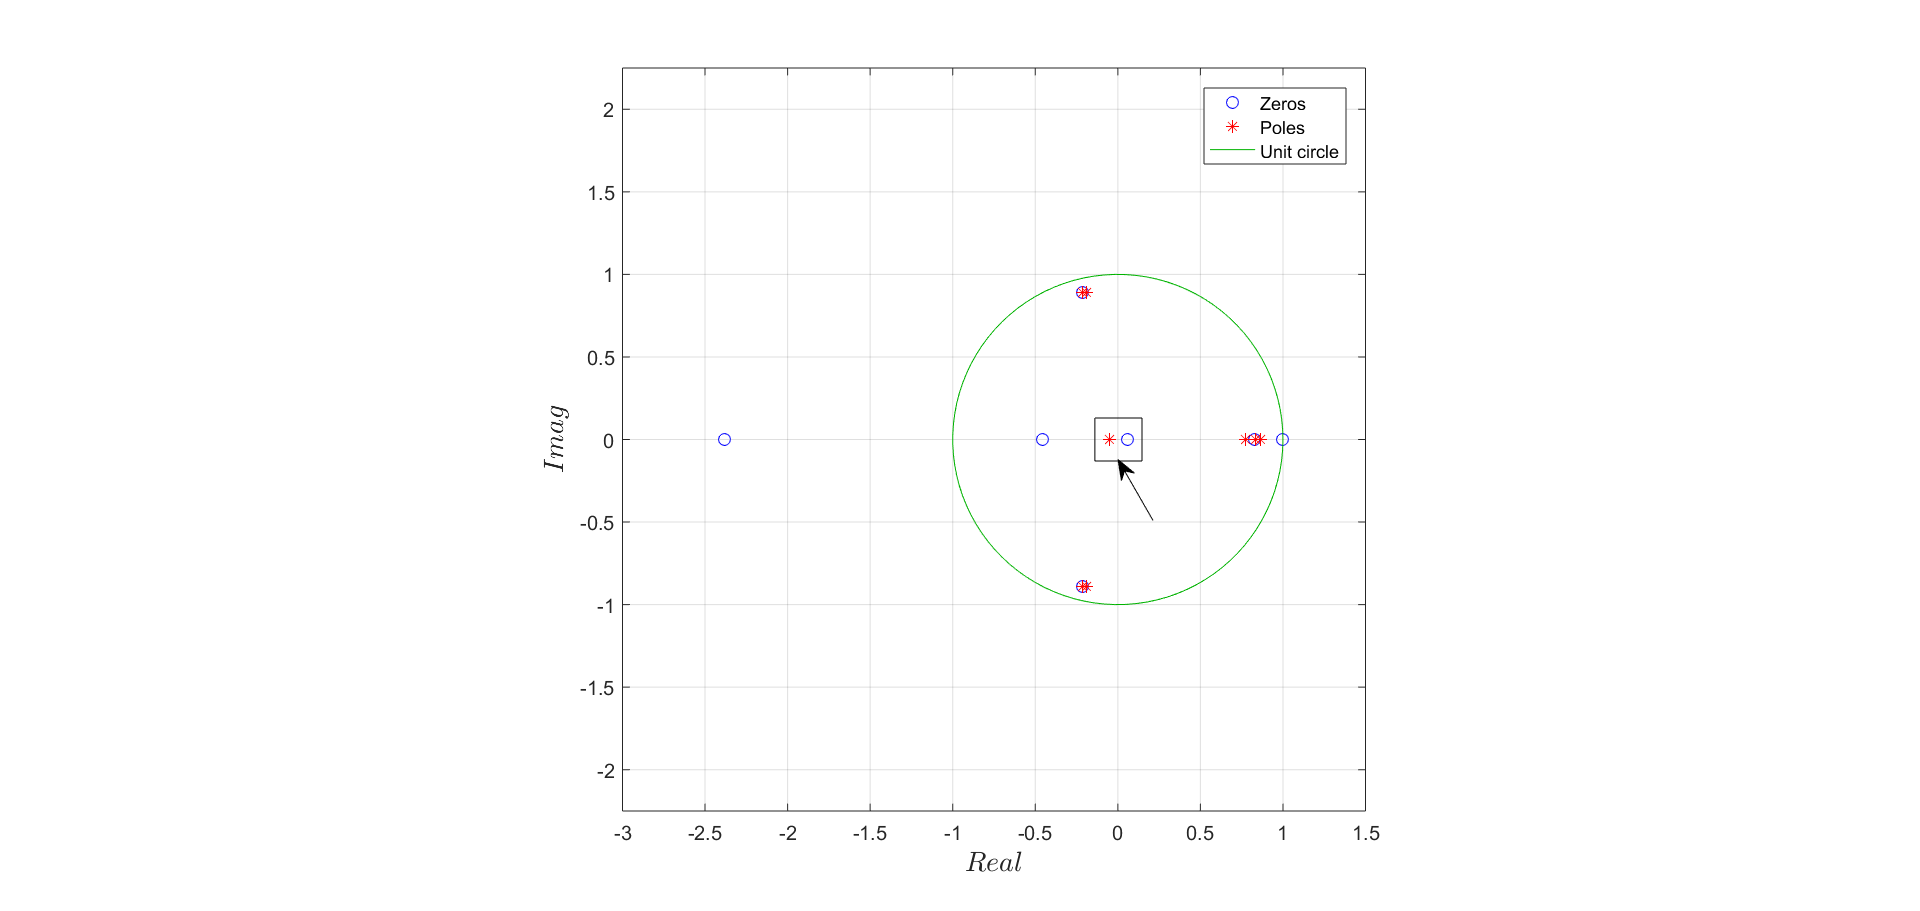
\includegraphics[scale=0.38,trim={4.5cm 0 0 0},clip]{task254.png}  
	\caption{eigenvalues/zeros of 8-state model for channel $(2,2)$}
	\label{task254} 
\end{figure} 
\clearpage
The eigenvalues/zeros of the model with $n_{s}=8$ are plotted in Fig. 16-19. When comparing these plots with the model with $n_{s}=7$, it can be clearly seen that the plots are very similar except that for the model with $n_{s}=8$, there is an additional pole/zero cancellation in each channel (shown with arrows). Hence, the 'extra' state dimension in the $n_{s} = 8$ case does not have much impact on the input-output properties of the system compared to the $n_{s} = 7$ model. Note that the locations of poles and zeros in the extra pole/zero cancellation are not exactly the same, but they very close in a sense the pole/zero cancellation can be confidently assumed.

\section{Correlation Functions}
\textbf{Task 3: Impulse response identification from white noise inputs}\\
A pulse input to a system is not always ideal in order to determine its impulse response because disturbances
and measurement noise also contribute to the observed outputs and, because of limitations on how large the
input magnitude can be, it may not be possible to increase the pulse height to a level where the system's
response is dominated by the effect of the pulse input. Thus, it is advantageous to use inputs which are
persistent since it is possible to transfer more energy to the system when limits on the input magnitude are
present (which is always the case in any real test environment). A persistent input which is quite useful
in this regard is "white noise". Hence, it this section we consider the inputs in the form of white noises to the system and then study the system's response in different ways. Again we have two-inputs in the form of white noises and also we have two output, totally four channels.

\vspace{30pt}
\textbf{1.}\\
In this part we are asked to examine the mean of each input sequence and verify that they are close to zero. This can be done in two different ways. In the first method we just use the command 'mean' in Matlab and obtain the mean of each input sequence. This results in calculation of the mean for input sequence ($u_{1}$) is -0.00097 and for input sequence ($u_{2}$) is 0.0013. As it can be seen they are approximately zero mean.

The other method is to compute $R_{uu}[k]$ for each channel according to:

\begin{equation}
R_{uu}[k] = \lim\limits_{p \to \infty}\frac{1}{2p}\sum_{q=-p}^{p} u_{k+q}u_{q}^{T} \in \textbf{C}^{n\times n} 
\tag{5}
\end{equation} 


and then show that $R_{uu}$ is equal to:

%\begin{gather*}
	\[	R_{uu}[k] = 
	\begin{cases}
	\tag{6}
	I& \text{if } k = 0\\
	0              & \text{if } k \neq 0
	\end{cases}
	\]% K^{2} \begin{bmatrix}
%	I & 0 \\
%	0 & I \\
%	\end{bmatrix} \tag{5}
%\end{gather*}

This would show that the input sequences are zero mean and unit variance. In this case, the different scalar channels of u are uncorrelated for all lag factors $k$ (the signals in each channel are typically called "independent" in this case).
Since this will be done in next parts, we just leave this method for now and discuss it later.\\

\vspace{20pt}
\textbf{2.}\\
In this section we are asked to to estimate the four entries of the $R_{uu}$ which can be calculated according to Eq. 5. the range of $k$ which is called the lag index should be $k \in [-200,200]$ corresponding to the lag factor $\tau \in [-5,5]$ second. This is plotted in Fig. \ref{task32}. As it can be seen from these plots, the $2\times2$ $R_uu[k]$ matrix is approximately equal to what is presented in Eq. 6 and hence we can conclude that it is zero mean but the variance is approximately 4. This will be discussed in the next part.

\begin{figure}[ht!]  
	\centering    
	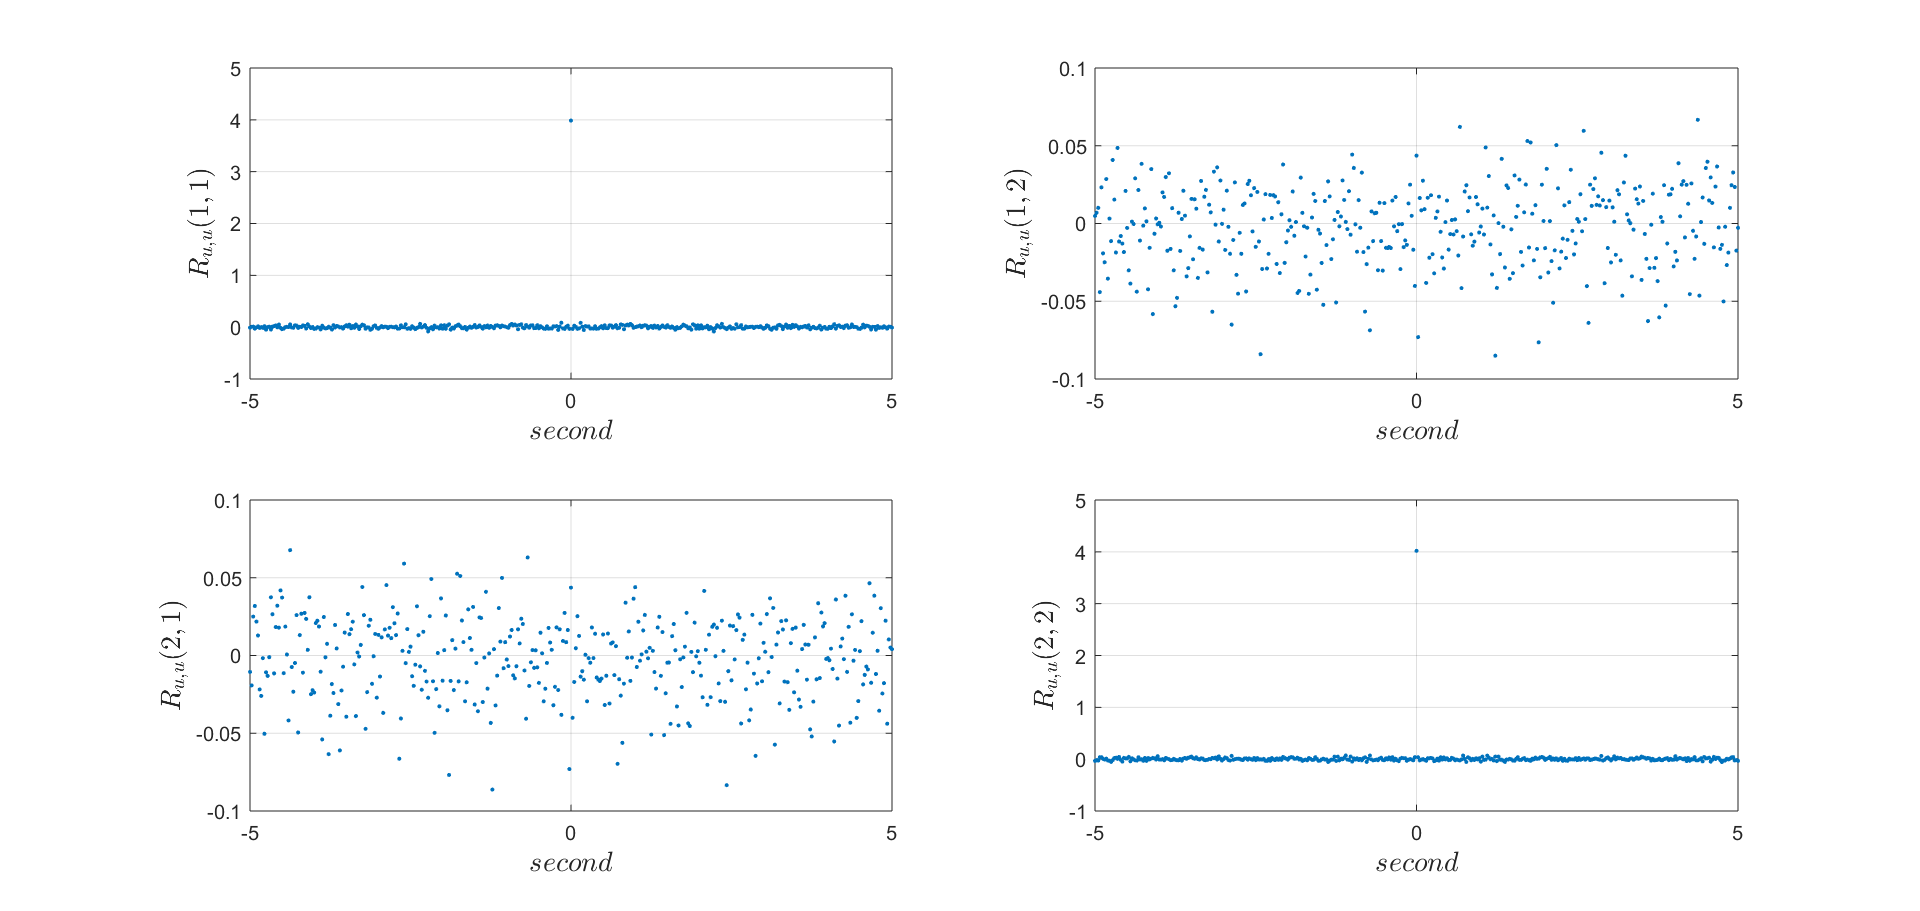
\includegraphics[scale=0.38,trim={4.5cm 0 0 0},clip]{task32.png}  
	\caption{Four entries of $R_{uu}$ for lag factor $\in [-5,5]$ second}
	\label{task32} 
\end{figure} 

\vspace{20pt}
\textbf{3.}\\
In this part we are asked to calculate auto-correlation of $u$ vector input with no lag, $R_{uu}[0]$. Using Eq. 5 and putting $k=0$, the result is:

\begin{gather*}
R_{uu}[0] = \begin{bmatrix}
3.9851    & 0.0436 \\
0.0436    & 4.0196 \\
\end{bmatrix} \tag{7}
\end{gather*}

As suggested by the question in this part, the $R_{uu}[k]$ can be approximated to:

\begin{gather*}
R_{uu}[0] \approx \begin{bmatrix}
4 & 0 \\
0 & 4 \\
\end{bmatrix} \tag{8}
\end{gather*}

and hence, the variance is approximately 4, and not 1. This is an important issue for the next part since we basically need to normalize the cross-correlation matrix data to estimate the impulse response of the system.

\vspace{20pt}
\textbf{4.}\\
Since we are dealing with asymptotically stable linear time-invariant system, if input $u$ produces output $y$, then $R_{uu}$ produces $R_{yu}$. Importantly, if input $u$ is zero-mean, unit variance white noise, then $R_{yu}[k] = h[k]$. Hence, in this part we are asked to compute the cross-correlation between input $u$ and output $y$ and then compare the results with the impulse response of the system. In this way, we are basically comparing how the system behave under different input conditions which are somehow related. Hence, the system's response should be close since in both cases the system has not changed. 
An important consideration here is that $R_{yu}[k] = h[k]$ only holds when the input noise has unit variance. In our data, as we calculated in previous parts, the variance is approximately 4 and hence $R_{yu}[k]$ needs to be scaled accordingly. The results are depicted in Fig. \ref{task34}. As it can be seen, the impulse response obtain from cross-correlation and actual system's response are very close.

\begin{figure}[t!]  
	\centering    
	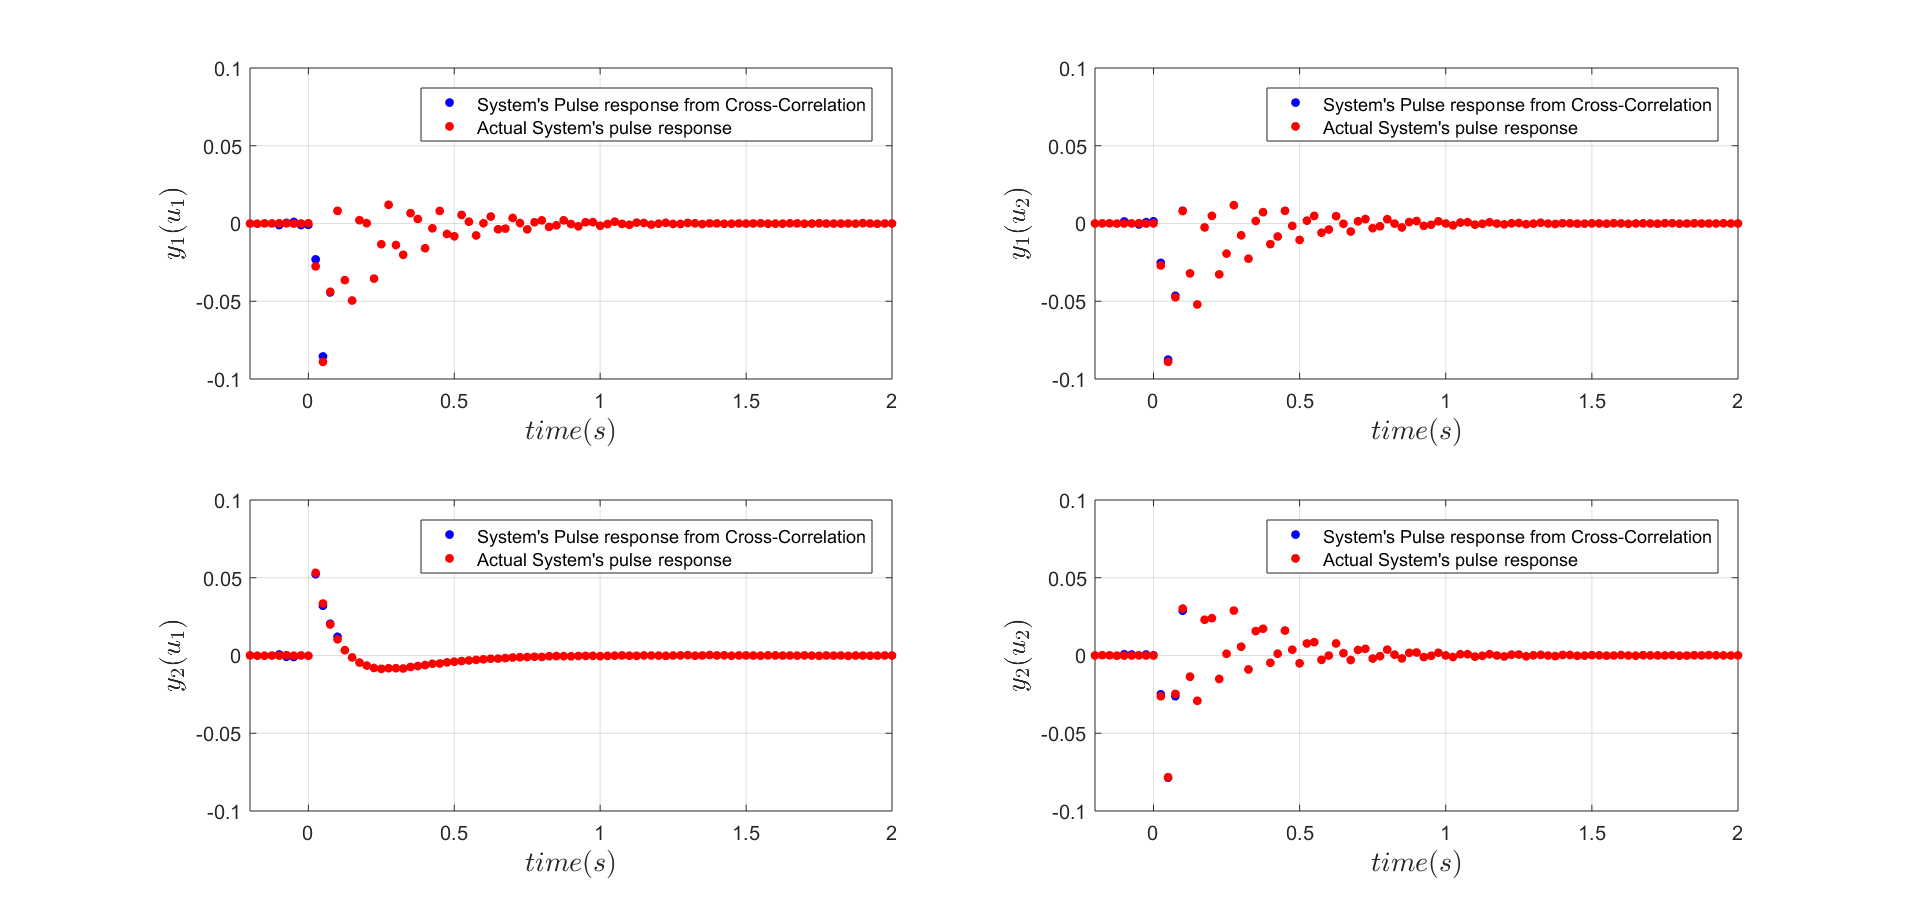
\includegraphics[scale=0.38,trim={4.5cm 0 0 0},clip]{task34.png}  
	\caption{Experimental impulse response obtained from
		the pulse response experiments vs. impulse responses computed from cross-correlation of noise response experiment}
	\label{task34} 
\end{figure} 

\section{System Norms}
\subsection{ $\mathcal{H}_{2}$ norm}
Just norms were defined for vectors and matrices, it is possible to define norms for systems and in this case,
the input "vectors" are actually drawn from some class of signals. Some of the system norms are induced
norms, and others are not. One major difference between signal and system norms compared to norms on finite dimensional vector spaces is that on finite dimensional vector spaces (including matrices) all norms
are equivalent in the sense that a vector that is small in one norm will also be small in another norm. This
does not generalize to norms on infinite dimensional vector spaces, i.e. linear spaces of signals and systems.

In this section, we want to compute the $\mathcal{H}_{2}$ norm of our discrete-time dynamic system from different methods and then compare the results together. Note that The $\mathcal{H}_{2}$ norm of a system is of great importance in control systems design because a typical objective is to design the controller so that the  $\mathcal{H}_{2}$ norm of certain closed-loop input-output channels in minimized.\\

\vspace{10pt}
\textbf{Task 4}\\
\textbf{1.}\\
In this section, we are asked to obtain the RMS value of the scaled output data $y$. Again, since the input sequence did not have the unit variance, we need to scale our input-output data by the factor of 2 (since the variance is approximately 4) and then compute the RMS (root mean square). The RMS value of a discrete-time signal v is defined as: 

\begin{equation}
||\text{v}||_{RMS}^{2} = \lim\limits_{p \to \infty}\frac{1}{2p}\sum_{q=-p}^{p} ||\text{v}_{k}||^{2}_{2}
\tag{9}
\end{equation} 

By simplifying Eq. 9 for the RMS value of the output $y$, we obtain new relations for the calculation of RMS of $y$ based on auto-correlation of y signal:

\begin{equation}
||\text{y}||_{RMS}^{2} = \lim\limits_{p \to \infty}\frac{1}{2p}\sum_{q=-p}^{p} tr(\text{y}_{k}\text{y}_{k}^{T})=tr\bigg(\lim\limits_{p \to \infty}\frac{1}{2p}\sum_{q=-p}^{p} \text{y}_{k}\text{y}_{k}^{T}\bigg) = tr(R_{\text{y}\text{y}}[0])
\tag{10}
\end{equation}
 
 Eq. 10 was used to calculate the $||\text{y}||_{RMS}$. The results is:
 
 \begin{equation}
 \tag{11}
 	||\text{y}||_{RMS} = 0.2237
 \end{equation}
 
 It can be shown that $||\text{y}||_{RMS}$ is equal to $\mathcal{H}_{2}$. In the next parts we are calculating $\mathcal{H}_{2}$ and then compare the results with $||\text{y}||_{RMS}$ that calculate in this part.

\vspace{20pt}
\textbf{2.}\\
In this part, we are asked to calculate $\mathcal{H}_{2}$ based on the 7-state model derived from the Hankel matrix analysis. It can be shown that for a discrete-time system that is causal, asymptotically stable, and has the state-space realization of $x_{k+1} = Ax_{k}+Bu_{k}$, $y_{k}=Cx_{k}$

\begin{equation}
	||P||^{2}_{\mathcal{H}_{2}} = tr\bigg(B^{T}G_{o}(\infty)B\bigg)=tr\bigg(CG_{c}(\infty)C^{T}\bigg)
	\tag{12}
\end{equation}

while the Gramians can be obtained according to the corresponding discrete-time Lyapunov equations:

\begin{gather*}
	A^{T}G_{o}(\infty)A-G_{o}(\infty) = -C^{T}C \tag{13} \\
	A^{T}G_{c}(\infty)A_{T}-G_{c}(\infty) = -BB^{T}
	\tag{14}
\end{gather*}

using Eq. 13 and Eq. 14, the observability and controllability Gramians are obtained as:

\begin{gather*}
	G_{c}(\infty) =	G_{o}(\infty) = \begin{bmatrix}
	0.29 &   0  & 0  &  0 &  0 &   0  & 0\\
	 0 &  0.26 &  0  & 0  &  0 &  0  &  0\\
	0  & 0 &   0.20  &  0 & 0 &  0 & 0\\
	 0  & 0  &  0  &  0.14  & 0 &  0  &  0\\
	0  & 0  & 0 & 0  &  0.11 &  0  & 0\\
	0 & 0  & 0  & 0  & 0 &   0.1 & 0\\
	0  &  0 & 0  &  0  & 0 &  0  &  0.07\\	
	\end{bmatrix}\\
\end{gather*}

As it can be seen, the observability and controllability Gramians are equal in this balanced coordinate frame and for this realization. Using Eq. 12, we obtain $||P||_{\mathcal{H}_{2}}$ as follows:

\begin{gather*}
	||P||_{\mathcal{H}_{2}} = 0.2297
\end{gather*}

\vspace{20pt}
\textbf{3.}\\
In this part, we are asked to compute $||P||_{\mathcal{H}_{2}}$ based on the experimental pulse response only (no model). For this, the following relation for $||P||_{\mathcal{H}_{2}}$ was used:

\begin{equation}
||P||^{2}_{\mathcal{H}_{2}} = \sum_{k=0}^{\infty} ||h_{k}||_{F}^{2}, \text{      } \text{      } h_{k}\text{ = discrete-time pulse response:}
\tag{15}
\end{equation}

Using Eq. 15 and the command 'norm' with the input of the actual pulse response matrix $h$ and another input of 'fro' (Frobenius norm option), we calculate $||P||_{\mathcal{H}_{2}}$ as follows:


\begin{gather*}
||P||_{\mathcal{H}_{2}} = 0.2298
\end{gather*}

Note that all values are very close to each other. One reason for the fact that $||\text{y}||_{RMS}$ yields slightly smaller results could come from the fact that we have normalized the input-output data by a factor of 2 while, as we computed, the actual variance is not 4 for inputs which is an error source. Nevertheless, the results can be considered acceptable and very close to each other.

\subsection{$\mathcal{H}_{\infty}$ norm}
The problem with $\mathcal{H}_{2}$ is that it is not an induced norm and does not satisfy the submultiplicative property. This property makes the $\mathcal{H}_{2}$ norm unsuitable for addressing another critical aspect of control systems design, namely, the robustness of the controller to perturbations of the plant dynamics. The $\mathcal{H}_{\infty}$ norm of an asymptotically stable linear system P is defined as:

\begin{gather*}
	 ||P||_{\mathcal{H}_{\infty}} = \sup_{w}\overline{\sigma}(P(jw))
\end{gather*}

In this section, we are basically asked to obtain $\mathcal{H}_{\infty}$ of the 7-state model that we have for the system. In this regard, we first calculate $\mathcal{H}_{\infty}$ for the continuous-time linear dynamic system. For the case of discrete-time linear dynamic system, we basically obtain the 'equivalent' continuous-time system matrices from those of discrete-time and then use the same formula that we obtained for the continuous-time system. Note that the continuous-time system has no direct physical meaning - it is merely constructed so that it's frequency response function at any given has a unique match with the physical discrete-time system's frequency response.

\vspace{20pt}
\textbf{1.}\\
In this section, we are asked to write a Matlab function that accepts as inputs the state-space matrices of a continuous-time system,
upper and lower limits for the search, and a tolerance, and then returns the $\mathcal{H}_{\infty}$ norm of the system within the specified tolerance, and the approximate frequency at which the maximum
gain is achieved. The Matlab function was written based on the algorithm explained in the project. Basically, the closed loop matrix $A_{clp}(\gamma)$ is first calculated at each increment step of $\gamma$ and then the eigenvalues of this $A_{clp}(\gamma)$ are calculated. If there exists $\gamma$ such that:

\begin{equation*}
||P||_{\mathcal{H}_{\infty}} \geq \gamma \iff \text{there exists a purely imaginary eigenvalue(s) of $A_{clp}(\gamma)$}
\end{equation*}

or equivalently

\begin{equation*}
||P||_{\mathcal{H}_{\infty}} < \gamma \iff \text{there exists no purely imaginary eigenvalues of $A_{clp}(\gamma)$}
\end{equation*}

then we pick $||P||_{\mathcal{H}_{\infty}}$ to be $\gamma$. This function was tested with some matrices and then the results were compared to the $||P||_{\mathcal{H}_{\infty}}$ calculated from built-in Matlab functions. There results confirmed that our function performs well and very close to the output of the Matlab built-in function. The code will be included in the submission of our Matlab code for this project.

\vspace{20pt}
\textbf{2.}\\
In this part, we are essentially asked to do the same thing as the previous part, but with the difference that $||P||_{\mathcal{H}_{\infty}}$ should be obtained for the discrete-time linear system. In this case, we first obtain the 'equivalent' system matrices and frequencies to those of continuous-time system and then use the function we developed in the previous part to calculate the $||P||_{\mathcal{H}_{\infty}}$ of the discrete-time system. One challenging part to develop this code was to come up with appropriate matrices so that 'equivalent' continuous-time matrices be appropriate matrices which would return bounded $||P||_{\mathcal{H}_{\infty}}$ and we could confirm the performance of our functions. A good selection for discrete-time matrices was obtained using Matlab and then the results were compared to the Matlab built-in function. Similar to previous one, the performance of the function calculating $||P||_{\mathcal{H}_{\infty}}$ for discrete-time system is well and very close to that output of the Matlab built-in function. The code will be included in the submission of our Matlab code for this project.

\vspace{20pt}
\textbf{3.}\\
In this section, we are asked to use the previous functions we have already wrote and based on these calculate the $\mathcal{H}_{\infty}$ norm of our 7-state discrete-time model as well as specifying
the frequency at which it is achieved. The results are:

\begin{gather*}
	||P||_{\mathcal{H}_{\infty}} = 0.4723 \\
	 \omega_{0} = 71.15 \text{ Rad/s } 
\end{gather*}

If we use the command '[ninf,fpeak] = hinfnorm(sys)' for our system, the results will be very close.

\vspace{20pt}
\textbf{4.}\\
In the last part, we are asked to compute the discrete-time frequency response of the identified 7-state model on a frequency grid in the interval
$[0,\omega_{nyq}]$ and then plot the singular values of the frequency response at each frequency. Note that the frequency response matrix of the system is a $2\times2$ matrix and hence two singular values will be obtained at each frequency. Overlay on top of the singular values, the singular values that we compute from the empirical frequency response data are plotted. Finally, we plot the $\mathcal{H}_{\infty}$ norm computed from the model which locates the magnitude and corresponding frequency as a single point in this graph. The resultant plot is shown in Fig. 22.

As it can be seen, the model singular values are very close to the empirical singular values
and that the $\mathcal{H}_{\infty}$ norm computed from the model locates the magnitude and corresponding frequency
where the maximum singular value achieves its largest value.

\begin{figure}[t!]  
	\centering    
	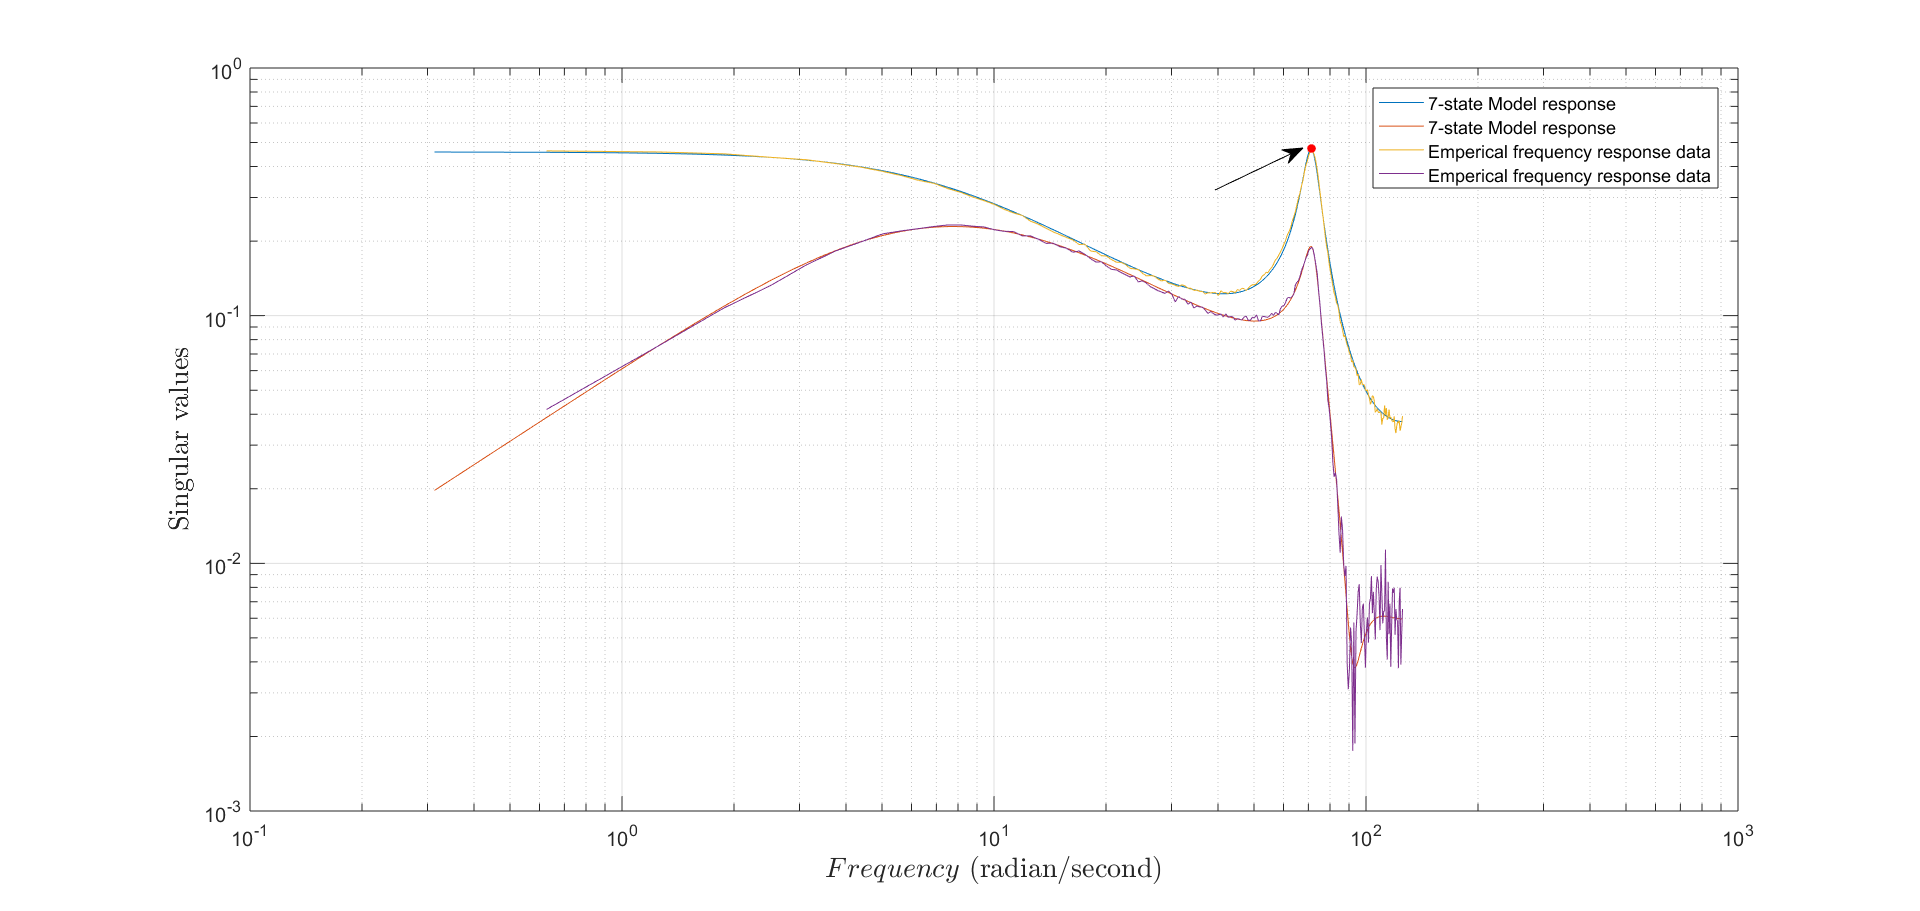
\includegraphics[scale=0.38,trim={4.5cm 0 0 0},clip]{task54.png}  
	\caption{Singular values of frequency response obtained for modeled vs. actual system.}
	\label{task34} 
\end{figure} 

\end{document}